\documentclass[letterpaper,12pt,oneside]{book}

\usepackage[utf8]{inputenc}
\usepackage[spanish,es-nodecimaldot,es-tabla]{babel}
\usepackage{graphicx}
\usepackage{multirow}
\usepackage{natbib}  % Usando paquete para citas
\usepackage{amsmath} % Notación
\usepackage{amssymb}
\usepackage{amsthm}  % Definiciones
\usepackage{siunitx}
\usepackage{todonotes}   % insert [disable] to disable all notes
\usepackage[T1]{fontenc} % Required for accented characters
\usepackage{outlines}
\usepackage{url}
\usepackage{soul}  % Tachar caracteres
\usepackage{tipa} % Caracteres IPA
\usepackage{smartdiagram}
\usepackage{color, colortbl}
\usepackage{gb4e} % Glosa
\noautomath  % Solve problems with render pdf
% https://tex.stackexchange.com/questions/325621/gb4e-package-causing-capacity-errors

\definecolor{Yellow}{rgb}{1, 0.78, 0.26}

\newcommand{\note}[4][]{\todo[author=#2,color=#3,size=\scriptsize,fancyline,caption={},#1]{#4}} % default

%For comments in a bubble on the document margins:
\newcommand{\ximena}[2][]{\note[#1]{Ximena}{green!40}{#2}}
\newcommand{\vic}[2][]{\note[#1]{Vic}{orange!40}{#2}}
\newcommand{\diego}[2][]{\note[#1]{Diego}{blue!40}{#2}}

%For inline comments:
\newcommand{\Ximena}[2][]{\ximena[inline,#1]{#2}\noindent}
\newcommand{\Vic}[2][]{\vic[inline,#1]{#2}\noindent}
\newcommand{\Diego}[2][]{\diego[inline,#1]{#2}\noindent}

% For code formatting
\def\code#1{\texttt{#1}}

% Teoremas y ejemplos
\theoremstyle{definition}
\newtheorem{exmp}{Ejemplo}[section]
\newtheorem{definition}{Definición}

\graphicspath{{./img/}}

\begin{document}

\bibliographystyle{acl_natbib}  % Cargando estilo de bibliografia

\author{Diego Alberto Barriga Martínez}
\title{Etiquetador automático de la morfología del otomí usando predicción estructurada}
\maketitle
\tableofcontents


\chapter{Introducción}

% capítulo corto con el objetivo, hipótesis y tocar los temas del marco teorico de forma muy superficial. Se definen en el marco teorico

%\section{Lengua otomí}

%En esta sección se menciona los lugares donde se describe el idioma otomí de forma somera, se mencionan algunos lugares donde es hablado el otomí y características fundamentales de la lengua.

%\subsection{Origen}

\Ximena{Basarme en la entrada de Elotl para hablar del otomí}

% Pie de pagina, no meter cosas tangenicales. Citar esta definicion
%La palabra otomí es de origen náhuatl (singular: \textit{otomitl}, plural: \textit{otomí}). Por otra parte, los otomíes se nombran a sí mismos \textit{ñähñu}\footnote{Existen organizaciones indígenas, como el Consejo de la Nacionalidad Otomí, que escriben la auto-denominación como hñätho hñähñu y también ñätho ñähño. Sin embargo, esta auto denominación puede variar.}, que significa "los que hablan otomí".

%Los grupos indígenas que hablan el idioma otomí se encuentran en diversas partes del territorio mexicano como: Estado de México, Querétaro, Hidalgo, Puebla y Veracruz \citep{barrientos2004otomies}. El otomí es una lengua indígena una gran variación dialectal que depende de su distribución geográfica.

%En el Estado de México el pueblo \textit{ñähñu} está disperso por varios municipios tales como: Toluca, Lerma, Chapa de Mota, Aculco, Amanalco, Atizapán de Zaragoza, por mencionar algunos. En otros municipios como Naucalpan, Ecatepec, Nezahualcóyotl y Tlalnepantla se pueden encontrar hablantes por efectos de la migración. Según \citet{barrientos2004otomies} la población total de hablantes otomíes en el Estado de México supera los cien mil, sin embargo, datos actuales .

%En concreto existen \textbf{nueve} variantes del otomí y cabe recalcar que dicha variación puede presentarse incluso dentro del mismo estado. Tan solo el Estado de México presenta tres variantes del otomí: El otomí de Tilapa, hablado en el municipio de Santiago Tianguistenco; el Otomí de Acazulco, del municipio de San Jerónimo Acazulco; y el Otomí de Toluca, de San Andrés Cuexcontitlán.

\section{Problemática}

El NLP es un área de la computación que permite reconocer, procesar e interpretar el lenguaje humano dentro de un sistema computacional. El objetivo de esta área es hacer que las computadoras realicen tareas que involucran el lenguaje humano. Algunas tareas generales consisten en permitir la comunicación humano-máquina, o simplemente hacer un exitoso procesamiento de texto o voz humanos \citep{jurafsky2008speech}. Ejemplos de aplicación actuales son los traductores automáticos, asistentes personales que reconocen voz, motores de búsquedas en Internet, análisis de sentimientos en textos,  síntesis de voz, etiquetado de textos y muchas más aplicaciones.

% Voy de lo mas general a lo particular
Una de las tareas más populares de NLP es el etiquetado automático de textos. Este etiquetado puede realizarse a diferentes niveles lingüísticos, por ejemplo, morfosintáctico (\textit{Part Of Speech tagging, POS}), sintáctico (\textit{parsing}), morfológico, etc.  El nivel morfológico tiene que ver con la estructura interna de las palabras \citep{haspelmath2013understanding}; en particular, existe un tipo de etiquetado, de gran importancia para el análisis lingüístico, llamado glosado que asigna etiquetas a las unidades que conforman a una palabra. 

% Hablando de ML
Para lograr lo anterior, los enfoques actuales aplican técnicas de ML. El ML es un subcampo de la Inteligencia Artificial (IA), que constituye un enfoque de resolución de problemas caracterizado por estimar una solución a partir de la experiencia \citep{mitchell1997machine}.  La experiencia se refiere a datos etiquetados (ejemplos) que permiten inferir un modelo estadístico de aprendizaje. Entre los métodos de ML ampliamente utilizados se pueden mencionar las Support Vector Machines (SVMs), árboles de decisión, o bien los modelos gráficos, como las redes neuronales o los métodos generativos, solo por mencionar algunos. Para las tareas de etiquetado en \textit{NLP} generalmente se utilizan modelos gráficos supervisados, por ejemplo, modelos ocultos de Markov (\textit{Hidden Markov Models, HMM}).

% Introduccion de la problematica
No obstante, el lenguaje natural es complejo y dinámico, ya que tiene fenómenos que hacen que las tareas de reconocimiento, generación y procesamiento se vuelvan difíciles para las computadoras. Adicionalmente, existen escenarios donde estos métodos no son efectivos como es el caso de las lenguas de bajos recursos, que son lenguas que tienen pocos recursos digitales con los que trabajar. Por ejemplo, si se tienen pocos datos iniciales para el entrenamiento del modelo de aprendizaje las predicciones serán poco precisas o equivocadas. Los bajos recursos son un escenario común en México donde, a pesar de que existe una rica diversidad lingüística, gran parte de las lenguas originarias no poseen contenido web ni publicaciones digitales y por tanto carecen también de tecnologías del lenguaje.  El escenario mencionado anteriormente supone un reto para los métodos de aprendizaje convencionales, que requieren de grandes cantidades de datos de entrenamiento para funcionar correctamente. Por lo tanto, es un importante reto de investigación desarrollar aproximaciones que funcionen con lenguas de escasos recursos. En particular, en este trabajo nos enfocamos en el glosado automático del otomí, una lengua con gran riqueza morfológica y con escasez de recursos digitales.

El glosado puede ser un primer paso para el desarrollo de más tecnologías del lenguaje; no solo para el otomí, que presenta un grado de extinción acelerada (Comisión Nacional para el Desarrollo Indígena)\footnote{https://www.gob.mx/inpi/}, sino para las 68 agrupaciones lingüísticas que se hablan en México.

\section{Objetivo}

Diseñar e implementar un etiquetador morfológico para el otomí basado en técnicas de Procesamiento del Lenguaje Natural (\textit{Natural Language Processing, NLP}) con Aprendizaje de Máquina (\textit{Machine Learning, ML}). En particular, se hará énfasis en métodos de aprendizaje estructurado y supervisado. Específicamente, se aplicará \textit{Conditional Random Fields (CRF)} para etiquetado morfológico (glosado) del otomí, una lengua de bajos recursos.

\section{Hipótesis}

Se espera obtener un modelo que produzca glosa para el otomí, generada automáticamente, con base en el entrenamiento con pocos ejemplos previamente etiquetados. Al obtener una buena exactitud en la predicción automática de glosa se apoyaría a los anotadores humanos a reducir trabajo repetitivo y exhaustivo. Además, se espera obtener avances de una metodología adaptable a un mayor número de lenguas mexicanas. Sería deseable que esta metodología experimental pueda ser replícale en otras lenguas habladas en México.

% Marco teórico
\chapter{Avances en etiquetadores automáticos}\label{sec:marco}

% Mencionar los bajos recursos

En este capítulo se trataran conceptos fundamentales del \textit{Natural Language Processing (NLP)}, haciendo énfasis en los etiquetadores, y conceptos del \textit{ Machine Learning (ML)} con enfoque en los métodos de aprendizaje basados en gráficas. Para las últimas sub-secciones se abordará elementos de los \textit{CRFs} que serán de utilidad para la comprensión de la arquitectura propuesta en este trabajo.

% Se tiene que explicar los conceptos de low resouces 
% modelos gráficos

% Low resources
% Algoritmo L&BFGS
    % L1/L2

\subsection{Natural Language Processing (NLP)}

% Introduccion
Dentro de las ciencias de la computación existe una subrama llamada Inteligencia Artificial (IA). Para este trabajo podemos decir que la IA\footnote{Es preciso señalar que la definición de los objetivos y alcances de la IA es un tema del que aún no hay consenso dada la amplitud del área, la ambigüedad de conceptos como inteligencia y los diversos enfoques existentes como los centrados en el comportamiento o en el pensamiento.} se enfoca en la construcción de sistemas o agentes que perciben su entorno, operan de forma autónoma, se adaptan al cambio y crean o persiguen objetivos para obtener el mejor resultado, y cuando hay incertidumbre, el mejor resultado esperado \citep{russell2010artificial}.

% Introducir elementos del lenguaje ¿Lenguaje Humano?
% Definición del NLP

Dentro de la IA existe una disciplina llamada procesamiento de lenguaje natural (por sus siglas en inglés \textit{Natural Language Processing, NLP}) que busca hacer que las computadoras puedan entender el lenguaje natural en sus distintos niveles lingüísticos\footnote{1. fonético y fonológico, 2. morfológico, 3. morfosintáctico, 4. sintáctico, 5. semántico}\citep{victor2020pln}. En ese sentido, dependiendo de la aplicación o tarea a resolver las técnicas de \textit{NLP} se enfocan en uno o varios niveles lingüísticos. Puede ser desde tener noción de lo que es una palabras en un texto hasta que la computadora tenga un conocimiento semántico del lenguaje. % TODO: Refinar la ultima parte

% Las citas
En otras palabras, el \textit{NLP} se encarga del procesamiento de los fenómenos del lenguaje natural a través del tratamiento y análisis de textos o voz permitiendo que las computadoras realicen tareas que involucren elementos propios del estos lenguaje \citep{jurafsky2008speech}. \textit{NLP} tiene dos grandes enfoque que es el orientado a voz y orientado a texto. En esta tesis nos enfocamos en la representación textual del lenguaje.

%Es necesario aclarar que entenderemos al lenguaje natural como aquel que se manifiesta a través de sonidos producidos por los humanos o en textos escritos y que forman palabras, oraciones y discursos.

Debido a que  el tratamiento del lenguaje es complejo para las computadoras requiere la intervención de múltiples disciplinas por lo que el \textit{NLP} se convierte en un área multidisciplinaria. Ciencias de la computación, psicología, ingeniería, matemáticas, filosofía, ciencias cognitivas y lingüística, por mencionar algunas, son áreas del conocimiento relevantes para esta área. 

Esto obliga a recordar el trabajo de \citet{turing1950computing} dónde se plantea la pregunta "¿Pueden las máquinas pensar?'' y propone un ejercicio práctico, que después seria conocido como la prueba de Turing. Hoy en día aun es difícil saber si las computadoras pueden emular procesamiento del lenguaje en la mente, por lo que estos conceptos son abordador por las ciencias cognitivas y la filosofía. Comprender cómo es la representación de los elementos del lenguaje y cómo sucede su procesamiento en la mente humana podría suponer avances para que las computadoras hagan lo propio. 

%\Vic{¿Como influye la lingüística en el NLP?

En particular el \textit{NLP} se necesita de una relación estrecha entre la lingüística y la ingeniería en computación. La lingüística se encarga del estudio de la lengua en todas sus manifestaciones. Tradicionalmente se habla de diferentes niveles de la lengua que ayudan a su estudio, por ejemplo, la fonología, la morfología, la sintaxis, la semántica, la pragmática. La lingüística debe proveer los conocimientos fundamentales sobre la lengua, de tal forma que permita una representación formal de ésta para que se logre su procesamiento por una computadora.

% Hacer énfasis en cuestiones lingüísticas.
% Decir que la Lingüística computacional y NLP para mi son lo mismo aunque ciertos autores 

La lingüística en combinación con ingeniería en computación cobran un papel importante para el \textit{NLP} (también llamado lingüística computacional)\footnote{Para ciertos autores existe una distinción entre lingüística computacional y NLP pero en este trabajo las consideramos como sinónimos. Para profundizar en esta distinción ver: } \diego{TODO: cita de jurafsky y manning}. En la figura \ref{fig:compu_linguistics} muestra la intersección de disciplinas que hacen posible el desarrollo  del \textit{NLP} o lingüística computacional. Es importante recordar que mucho de los avances recientes han sido impulsados por el creciente poder computacional para el manejo de grandes cantidades de información.

\begin{figure}[ht]
	\centering
	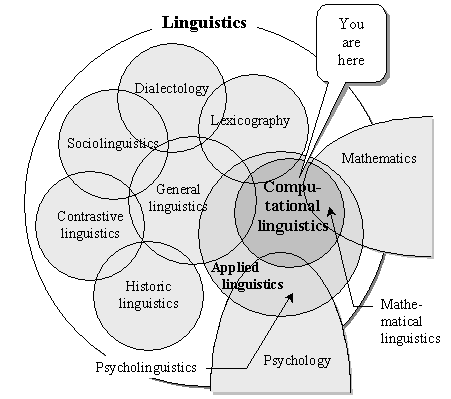
\includegraphics[scale=0.5]{computational_linguistics}
	\caption{Estructura de la ciencia lingüística \citep{bolshakov2004computational}}
	\label{fig:compu_linguistics}
\end{figure}

% Brevísima revisión histórica
Los primero enfoques de \textit{NLP} que trataron de lidiar con el lenguaje se basaron en modelos formales como máquinas de estados finitos, modelos basados en reglas, sistemas apoyados de lógica formal. Posteriormente comenzaron a aplicarse los modelos estadísticos, en particular los modelos de aprendizaje automático.

Dentro de los enfoques basados en reglas, uno de lo trabajos fundacionales pueden atribuirse a \citet{chomsky1956three}, dónde considera por primera vez a los autómatas finitos como una forma de caracterizar una gramática, y define un lenguaje finito como un lenguaje generado por una gramática finita (finite-state grammar). Estos primeros avances y los de otros fueron enfocados en la generación manual de reglas lingüísticas que intentaban modelar el lenguaje humano.

% Importante, comprender bien canal ruidoso
Por otra parte, se comenzó a implementar un enfoque estadístico que tiene raíces en diversos trabajos, uno de los más importante, el de \citet{shannon1948mathematical} basado en la teoría de la información. En estos modelos se recogen conceptos como canal ruidoso y decodificación para la transmisión del lenguaje a través de un medio. Se introduce el concepto de entropía como forma de medir la capacidad de un canal para transmitir información, o la información contenida por un lenguaje \citep{jurafsky2008speech}.

Con el paso de los años, el poder de cómputo y la accesibilidad a grandes cantidades de datos de provocaron que los métodos estadísticos, específicamente de \textit{ML}, cobraran gran relevancia. En este trabajo nos enfocaremos en estos métodos estadístico. En la subsección \ref{subsec:ml} se abundará más sobre el \textit{ML} y sus diversos enfoques.

% Mencionar los diferentes módulos o tareas que abarcan la disciplina. 
\Ximena{Extender las tareas del NLP. Darle un giro dramático. Hoy en dia es inegable que usamos productos de NLP. Buscar estadísticas de millones de personas que usan google translate}
\Ximena{Cerrar en grande. Hoy en dia las tareas son complicadas. Son tareas importantes.}

% NLP es difícil
Las tareas que aborda el \textit{NLP} son complicadas ya que, a diferencia de otros sistemas de procesamiento de datos, las aplicaciones que procesan el lenguaje necesitan utilizar ciertos conocimientos del lenguaje. Hay muchos retos en la creación de este tipo de aplicaciones. Por mencionar alguno, se utilizan este conocimiento para resolver cierto nivel de ambigüedad. Esto quiere decir que una frase puede tener múltiples significados dependiendo de factores como el contexto. Por ejemplo, ``El hombre ve a la mujer con el telescopio''. ¿Quien tiene el telescopio el hombre o la mujer? 

\Diego{¿Ejemplo?: ``Usted será afortunado si consigue que esta persona trabaje para usted''. ¿Afortunados por que la persona es buena trabajando o porque hacerla trabajar es un reto?}

% Cierre con aplicaciones actuales
A pesar del gran reto que representa que una computadora logre un procesamiento aceptable del lenguaje y sus fenómenos, gracias a los avances en investigación, es innegable que hoy en día utilizamos muchos productos de \textit{NLP} en la vida diaria. Algunos de estos productos son la traducción automática (Google translate, DeepL), síntesis y reconocimiento automático de voz (Siri, Cortana, Alexa), clasificación de documentos, sistemas de preguntas-respuestas (Google Assistant), buscadores (Duckduckgo, Bing, Google) y etiquetado automático de textos. El etiquetado automático es la tarea en la que se centra este trabajo. 

% Etiquetadores a nivel morfológico
%\Ximena{Refinar esta parte}
El etiquetado automático de textos consiste en predecir etiquetas o categorías que deberían llevar las partes de un texto, sean estas palabras, partes de palabras o frases completas. Se utiliza para realizar ciertos análisis lingüísticos y en \textit{NLP} agregar información no explicita en el texto para facilitar su desambigüación, por mencionar un ejemplo.

En concreto, en este trabajo se realizará un etiquetador automático de textos en otomí a nivel morfológico. Sobre la tarea de etiquetado automático será profundizada en la subsección \ref{subsec:taggers}.

% Machine learning
\subsection{Machine Learning (ML)} \label{subsec:ml}

El Aprendizaje de Máquina (por sus siglas en inglés \textit{Machine Learning (ML)}) es otra de las subrama de la IA que se forma a partir de la 
intersección de la estadística y las ciencias de la computación. El ML aborda la pregunta de cómo construir sistemas computacionales que automáticamente mejoren su desempeño en una tarea a través de la experiencia \citep{jordan2015machine}.

El estudio del \textit{ML} busca responder esta pregunta desarrollando modelos estadísticos con miras en la implementación de sistemas de software. En los últimos años, los resultados y avances del \textit{ML} han sido ampliamente adoptados y se pueden encontrar en sistemas de reconocimiento de voz, visión por computadora, control automático de robots, entre otros. También, en diversas áreas científicas como biología, cosmología y ciencias sociales, se utilizan métodos de \textit{ML} para el análisis de datos experimentales.

El campo de \textit{ML} permite que una computadora aprenda a automatizar tareas a partir de la observación de datos. A diferencia de las tareas convencionales que son resueltas por máquinas, dónde hay un algoritmo bien definido para su solución, estas tareas tienen la peculiaridad de no tener una solución o forma de automatización bien definida debido a su complejidad.

% ¿Porqué no es una tarea clara?
Por ejemplo, programar un filtro que distinga entre correo electrónico deseado (\textit{ham}) y no deseado (\textit{spam}) supone un reto ya que no hay reglas claras para su solución. Solo considerar ciertos elementos como el remitente, la extensión del correo, la fecha o la aparición de ciertas palabras podría fácilmente clasificar correos deseado en la bandeja de \textit{spam} y viceversa. Lo que se necesita entonces es una forma de que la computadora infiera patrones, relaciones y elementos que no son claros a simple vista.

Los métodos de \textit{ML} pueden entenderse métodos que buscan la solución óptima que se ajuste a los datos observados dentro de un espacio de posibles soluciones. Esta búsqueda es guiada por los datos previos y el programa tiene la finalidad optimizar cierta medida de rendimiento.

Formalmente \citet{mitchell1997machine} dice que \textit{una máquina ``aprende'' de una experiencia E con respecto a una tarea T y una medida de rendimiento P, si el rendimiento de las tareas T, medidas por el rendimiento P, mejora con la experiencia E}. 

% Retomando el ejemplo del spam para aclarar la definición de Mitchell
Entonces, un detector de \textit{spam}, que es la tarea, deberá mejorar su rendimiento, medido por el número de correos que clasificó correctamente, a través de la experiencia obtenida del análisis de los correo recibidos previamente. Notamos que para aplicar métodos de \textit{ML} necesitamos tener un problema de aprendizaje bien definido y para ello debemos identificar ciertos elementos como la tarea a resolver, la medida de desempeño a mejorar y la fuente de experiencia.

En cierto sentido, el \textit{ML} busca emular el aprendizaje humano, que usualmente surge de la observación y el análisis mas que de la memorización, de forma simplificada y no profunda. Determinar que método de aprendizaje es el adecuado para ciertas tareas dependerá en gran medida de la naturaleza del problema definida por la experiencia o datos de observación.

Para que el aprendizaje sea exitoso se necesita que la máquina logre generalizar a partir de una cantidad finita de ejemplos. Los métodos de \textit{ML} se ven beneficiados de grandes cantidades de datos y del poder de computo creciente de los últimos años. Comúnmente entre más grandes son los datos de observación mejores son los resultados. Pero se tiene que tener una muestra representativa que permita generalizar adecuadamente.

% 
La gran cantidad de datos requiere la consideracion del poder de computo y que tan bien aprendera la maquina a partir de la cantidad y el tipo de informacion.

Para ello se hacen uso de metodos puramente estadisticos para la toma de decisiones y para saber que tanta informacion es necesaria para que una computadora resuleva una tarea. Tambien se considera la complejidad computacional con lo que se responde si un problema es tratable por una computadora.

Optimización y una funcion objetivo que es la que se optimiza. Utilizar el tipico problema de F(X) =Y. una funcion donde existe en un espacio parametrico y se optimiza de diferentes formas.


\Vic{Hablar de como es que el ML con métodos puramente estadísticos se vuelve un problema de optimización de una función objetivo.}

%En general, se busca transformar los datos de entrada en una representación numérica para que sean más manejables para la computadora.
%Regresando al ejemplo del filtro de correos, para que el programa generalice podría analizar los correos previos, extraer y analizar las relaciones entre las palabras que contiene y cuando llegue un correo nuevo pueda decidir, con base en las palabras y otras características, si es deseado o no.

\Diego{En lugar de hablar de entrada y salida mejor hablar de conjuntos de datos representativos que sirven para crear el modelo de aprendizaje. Ese modelo se aplica a otro dataset de evaluación. Quiza usar una forma esquematica}


\Diego{Separar sobre la representacion del conjunto de datos y copmo se representan numericamente las features. Agregar la propuesta. Enfasis en el tamaño de los datasets y agergar low resources que es un reto para ML}

\Diego{Si es un dataset anotado es Superviser learning, si no es etiquetado es Unsupervised learning}
    
%Una característica importante del \textit{dataset} es el tamaño. Comúnmente entre más grande es el \textit{dataset} mejores son los resultados. Pero se tiene que tener una muestra representativa que permita generalizar adecuadamente. En general, se busca transformar los datos de entrada en una representación numérica para que sean más manejables para la computadora. \diego{Mencionar el mapeo de la realidad a los numeros. ¿Porque se usa esta representación?} Esta representación numérica es llamada vector de características.

\Diego{Podría esquematizarlo en pasos}
% Haer un diagrama del modelo de aprendizaje
% Funcion de evaluacion: Dice que tanto generaliza la maquina
% Funcion objetivo: Funcion que minimizamos o maximizamos. Ayuda a estimar los pesos de la red o a estimar el arbol

%Para poder medir si hubo alguna mejora en el desempeño se utiliza una notación matemática formal llamada \textbf{funciones objetivo}. Estas funciones se encargan de decir que tan bueno o malo es el modelo en turno resolviendo una tarea.

% Hablar de train y test

% Tipos de ML
%Ya que existe una gran diversidad de tareas surgen varios enfoques dentro del \textit{ML} con los que algunas de estas tareas serán más sencillas de resolver que otras. Primero, esta el \textit{Supervised Learning} dónde se busca predecir etiquetas, generalmente expresadas como $y$, dado un vector de características de entrada, generalmente expresado como $x$. Work in progress...

% 2. Supervisado -> (enfocarme mas en esto)
% 4. Problemas secuenciales: Hablar de los problemas de secuencia y secuencia. Hay diferentes tipos de salidas. Por que son útiles en ML las secuencias.
% 1. No supervisado
% 3. Reinforcement 


% Diferencia entre modelos graficos y modelos secuancianciales. Hay una tarea enm que entra una tarea y se produce una secuencia de salida

\subsection{Etiquetadores} \label{subsec:taggers}

% Por qué es importante el etiquetado
% Buscar Morfologhical Parsing
% POS, NER, Etiquetado morfológico
% etiquetadores a diferentes niveles lingüísticos
% Teoría de etiquetado
% Seq2seq
% Que es la morfología 
% que es la glosa
% Que es un etiquetador
% Tipos de etiquetados
% Bio Labels
% Centrarnos en el glosado automatico
% =Que es el etiquetado de glosa? (Menos tecnico)
% Perspectiva general y divulgativa con la glosa
% Glosa automática

\subsection{Modelos gráficos}
% Aqui va lo mas pesado
% profundizar en los CRFs
% Los límites de los modelos gráficos para bajos recursos

% Cierre de los modelos gráficos y comenzar a hablar de CRF
% No perder de vista que los CRFs son modelos gráficos pero con ventajas

\subsubsection{Los límites de los modelos gráficos en para bajos recursos}

%A continuación se explicará qué ventajas tienen los \emph{Conditional Random Fields (CRF)} sobre otros modelos de aprendizaje, se mencionan formalmente los elementos fundamentales que describen los \emph{CRF's}.

En \textit{NLP} una tarea de interés es el etiquetado y segmentación de secuencias de datos. Para llevar a cabo esta tarea es habitual la utilización de \textbf{modelos generativos}, cómo los \textit{Hidden Markov Models (HMMs)}, o \textbf{modelos condicionales}, como los \textit{Maximum Entropy Markov Models (MEMMs)}.

Por una parte, los modelos generativos intentan modelar una probabilidad conjunta $P(x,y)$ sobre observaciones y etiquetas. Para definir esta probabilidad conjunta se necesita enumerar todas las observaciones posibles. Las limitantes de este enfoque son de diversas índoles como las grandes dimensionalidades en el vector de entrada $X$, la dificultad de representar múltiples características que interactúan unas con otras y dependencias complejas que hacen la construcción de la distribución de probabilidad un problema intratable con un enfoque computacional.

Por otro lado, una solución a las limitantes de los modelos generativos es un modelo condicional. Estos modelos no son tan estrictos como los primeros al momento de asumir independencias en las observaciones. Los modelos condicionales especifican la probabilidad de posibles etiquetas dada una secuencia de observación.

Consecuencia de lo anterior, no se gasta esfuerzo en modelar las observaciones, dado que en al momento de realizar pruebas estas observaciones son fijas. Segundo, la probabilidad condicional puede depender de características arbitrarias y no dependientes de la secuencia de observación sin forzar al modelo a tomar en cuenta la distribución de estas características, permitiendo que el modelo sea tratable \citep{lafferty2001conditional}.

Un ejemplo de estas ventajas con los \textit{MEMMs} que son modelos secuenciales de probabilidad condicional. Sin embargo, estos modelos y otros que son no generativos, de estados finitos y que son clasificadores basados en el estado siguiente comparten una debilidad llamada \emph{label bias problem}. \citet{lafferty2001conditional} define que existe el \emph{label bias problem} cuando "las transiciones que dejan un estado compiten solo entre sí, en lugar de entre todas las demás transiciones en el modelo".

Dado que las transiciones son las probabilidades condicionales de los siguientes posibles estados una observación puede afectar cuál será el estado siguiente sin tomar en cuenta que tan adecuado será este. Por tanto, se tendrá un sesgo en los estados con menos transiciones de salida.

\subsection{Conditional Random Fields}

Como menciona \citet{sutton2012introduction} modelar las dependencias entre las entrada puede conducir a modelos intratables, pero ignorar estas dependencias puede reducir el rendimiento.

Dado el que problema abordado en este trabajo, dónde se requiere del etiquetado de secuencias y es en contexto de bajos recursos lingüísticos, se hace necesario utilizar un enfoque más conveniente.

Los \textit{Conditional Random Fields (CRFs)} son un framework para la creación de modelos probabilístico utilizado en técnicas de aprendizaje estructurado. Tienen las ventajas de los \textit{MEMMs} y, en principio, solucionan el \emph{label bias problem}. El framework tiene un solo modelo exponencial para la probabilidad conjunta de todas las secuencias de las etiquetas de salida dada la secuencia de observación. En contraste los \emph{MEMMs} usan modelos exponenciales para cada probabilidad condicional de los estados siguientes dado el estado actual.

Formalmente \citet{lafferty2001conditional} definen los \textit{CRFs} como a continuacion se enuncia:

\begin{definition}
	Sea $G = (V,E)$ una gráfica tal que $\mathbf{Y} = (\mathbf{Y}_{v})_{v \in V}$, entonces esa $\mathbf{Y}$ es indexada por los vertices de $G$. Entonces $(\mathbf{X}, \mathbf{Y})$ es un \textsf{conditional random field} en caso de que las variables aleatorias $\mathbf{Y}$ se condicionen por $\mathbf{X}$, la variable aleatoria $\mathbf{Y}_{v}$ cumple la \textit{propiedad de Markov} con respecto a la gráfica: $p(\mathbf{Y}_{v}|\mathbf{X},\mathbf{Y}_{w},w \ne v) = p(\mathbf{Y}_{v}|\mathbf{X},\mathbf{Y}_{w},w \sim v)$, dónde $w \sim v$ significa que $w$ y $v$ son vecinos en $G$.
\end{definition}

En esta tesis, para el modelado de secuencias, se utiliza la forma más sencilla de la gráfica $G$ dónde es una cadena simple o línea. Esto quiere decir que $G = (V = \{1,2,...m\}, E = \{(i,i+1)\})$. A este tipo de \textit{CRFs} se les conoce como \textit{linear-chain CRFs}. Como menciona \citet{lafferty2001conditional} "si la gráfica $G = (V,E)$ de $\mathbf{Y}$ es un árbol (del cual una cadena es el ejemplo más sencillo), los \textit{cliques} son los límites y vertices. Entonces, por el teorema de los \textit{random fields} \citep{hammersley1971markov}, la distribución conjunta sobre las etiquetas de secuencias $\mathbf{Y}$ y $\mathbf{X}$ tiene la forma:

% TODO: Explicar esta ecuacion sobre que es son las lambdas, porque hay dos sumandos, porque el símbolo de proporcionalidad. Entre \proto y \bigg habia un \exp que hacia que se rompiera la ecuacion
\begin{equation}
    p{_{\theta}}(y|x) \propto \bigg( \sum\limits_{e \in \mathbf{E},k} \lambda_{k}f_{k}(e,\mathbf{y}|_{e},\mathbf{x}) + \sum\limits_{v \in \mathbf{V},k}\mu_{k}g_{k}(v,\mathbf{y}|_{v},\mathbf{x}) \bigg)
\end{equation}

% TODO: Mencionar la ecucacion
% TODO: Descripcion de la estimacion de parametros y característica de la función de perdida

De la ecuación  se destacan $f_{k}$ y $g_{k}$ que representan las \textit{feature functions}. Estas están definidas y son fijas. Las \textit{feature functions} de está tesis serán descritas más adelante. 


\section{Estado del arte}

% Por revisar
%Un ejemplo de desarrollo de modelos para lenguas de bajo recursos es el trabajo de Moeller y Hulden (2018) donde se realizó un glosador automático con alrededor de 3,000 palabras para la lengua naj-daguestaní llamada Lezgi. Otro trabajo relacionado es el de Anastasopoulos et al. (2018) donde se exploran métodos computacionales para anotar una lengua en peligro de extinción llamada Griko con etiquetas POS.

Los \textit{CRFs} han sido utilizados para la clasificación de regiones en una imagen, estimar el puntaje en un juego de Go, segmentar genes en una hebra de ADN y análisis sintáctico de lenguaje natural en un texto por mencionar algunas \citep{sutton2012introduction}.


\subsection{Trabajos sobre bajos recursos}
% Hablar del trabajo para Lezgi
Con base en el trabajo previo de \citep{moeller2018automatic} donde se utilizan técnicas de NLP y ML para tratar para el idioma Lezgi se plantea como hipótesis que dado el tamaño del corpus y la glosa que contiene 
se obtendrá texto correctamente glosado con una precisión de al menos 80\%.

\Diego{Descripción de la estimación de parámetros y característica de la función de perdida}
% Papers que hablen del tema de etiquetado automático 2010 para acá

% Redes neuronales,
% Mención de trabajo y papers actuales hacen algo similar

%%%%%%%%%%%%%%%%%%%%%%%%%%%%%%%%%%%%%%%%%%%%%%%%%%%%%
% Metodología                                       %
%%%%%%%%%%%%%%%%%%%%%%%%%%%%%%%%%%%%%%%%%%%%%%%%%%%%%

\chapter{Etiquetador morfológico para el otomí} \label{chap:metodology}

\Diego{¿agregar los baseline neuronales? paper NAACL}

El objetivo de este capítulo es la presentación de la metodología utilizada en esta tesis. La metodología está constituida por un corpus etiquetado, del cual se incluye una descripción detallada, y la arquitectura para la generación de glosa para el idioma otomí. La arquitectura incluye, entre otras cosas, la codificación y preprocesamiento del corpus, el diseño e implementación del los \textit{CRFs} y la determinación de las \textit{feature functions}.

El punto principal de la metodología fue la implementación de los \textit{CRFs} que mostraron claras ventajas sobre otros métodos de aprendizaje basados en gráficas. Elegimos este \textit{framework} ya que se presenta como una opción para el contexto de los bajos recursos digitales que presenta el otomí, como se describirá más adelante. En ese sentido, la implementación de los \textit{CRFs} fue utilizada para predecir secuencias de etiquetas, con el enfoque del aprendizaje estructurado, que describen las unidades morfológicas dentro de una palabra de una variante del otomí. 

% Particularidades del corpus (Análisis cualitativo y cuantitativo)
\section{Corpus: otomí de Toluca}

% Tipo de otomi y características de la variante
La clasificación lingüística introduce al otomí dentro de las lenguas otomianas, las cuales a su vez pertenecen a la rama otopame de la familia otomangue \citep{barrientos2004otomies}. Cada variante muestra particularidades fonológicas, morfológicas, sintácticas y léxicas. En el tratamiento de textos por medio de técnicas de \textit{NLP} se requiere que estos textos estén normalizados y homogéneos. Dicha normalización propicia la obtención del mejor desempeño posible en los diversos métodos de aprendizaje automático. Más adelante se describirá el proceso de preprocesamiento aplicado al corpus que tuvo el propósito de adecuar el corpus a la arquitectura y normalizar el texto.

% Otomi en general, Familia y rama
Esta  tesis utilizó un corpus en otomí que, además, cumple la característica de estar glosado. Se trabajó con la variante del otomí de Toluca de la región de San Andrés Cuexcontitlan.

% De donde vienen los textos, quien lo glosa y quien lo recolecta
Se recogió un corpus basado en el trabajo de \citet{lastra1992otomi} titulado \emph{El otomí de Toluca} y que a su vez fue etiquetado y glosado manualmente por el lingüista Víctor Germán Mijangos de la Cruz\footnote{TODO: Liga del repo}. Este corpus es un subconjunto del corpus paralelo español-otomi que se encuentra en la plataforma web Tsunkua\footnote{https://tsunkua.elotl.mx/}.

% Tokens y tipos de Palabras

% Numero de etiquetas diferentes
\begin{table}
	\centering
	\begin{tabular}{| c | c |}\hline
		\textbf{Categoría} & \textbf{Cuenta} \\ \hline
		Tokens (POS) & 8550\\
		Tipos (POS) & 44\\
		Tokens (Glosa) & 14405\\
		Tipos (Glosa) & 112\\
		\textbf{Total de oraciones etiquetadas} & \textbf{1769} \\ \hline
	\end{tabular}
	\caption{Tamaño del corpus}
	\label{table:corpus_length:1}
\end{table}

Además, se agregaron 81 lineas de casos poco usuales que son fenómenos poco frecuentes y, por tanto, particularmente difíciles de predecir. El subconjunto del corpus utilizado en la sección experimental está descrito en la tabla \ref{table:corpus_length:1}, donde se encuentra el tamaño de las etiquetas POS y el tamaño de la glosa y en la tabla \ref{table:corpus_text:1}, donde se puede ver los tipos de textos presentes en el corpus.

Los textos que componen el corpus fueron construidos a partir de las aportaciones de diez hablantes distintos de entre diez y setenta y tres años, de los cuales, siete son de sexo femenino y tres masculino \citep{lastra1992otomi}.

\begin{table}
	\centering
	\begin{tabular}{| c | c |}\hline
		\textbf{Textos} & \textbf{Número} \\ \hline
		Narrativos & 32 \\
		Dialogados & 4  \\
		\textbf{Total de textos}  & \textbf{36} \\\hline
	\end{tabular}
	\caption{Textos del corpus}
	\label{table:corpus_text:1}
\end{table}

% Citar el estándar de etiquetas https://www.eva.mpg.de/lingua/pdf/Glossing&Rules.pdf
Los tipos de etiquetas \textit{POS} presentes en el corpus se pueden observar en la tabla \ref{table:pos_types}. Dentro del corpus se encontrón glosas que no corresponden a etiquetas \textit{POS}, sino que describen la semántica (traducciones) de las palabras. Como por ejemplo: en el fragmento en otomí \textsf{"...ná ra sapahtá pe lo prinsipal..."} ("...empezado un Zapata, pero lo principa...") \textsf{sapahtá} tendría como glosa la palabra \textsf{zapata} que es su traducción. Esta forma de presentar las etiquetas \textit{POS} es común en el uso lingüístico y no vale la pena presentarla en la tabla \ref{table:pos_types} pues son descriptivos por sí mismos. 

\begin{table}
	\centering
	\begin{tabular}{| c | c | c | c | c |}
		\hline
		v & obl & det & cnj & dem \\ 
		unkwn & n & neg & p.loc & prt \\
		conj.adv & dim & gen & cond & it \\
	    lim & aff & loc & dec & conj  \\
	    cord & san & cnj.adv & regular/v & adv \\
	    adj & & & & \\
	    \hline
	\end{tabular}
	\caption{Tipos de etiquetas \textit{POS}} 
	\label{table:pos_types}
\end{table}

Por otra parte, presentamos una descripción de las etiquetas \textit{POS} en la tabla \ref{table:pos_descr} dónde se muestra el significado de cada una. Por último, la distribución de las etiquetas \textit{POS}, se encuentra en la figura \ref{fig:pos_distrib}. En esta figura se muestra una carga importante hacia unas pocas etiquetas \textit{POS}. Esta característica es considerara por el modelo de aprendizaje estructurado que utilizamos y puede suponer un problema importante en métodos de aprendizaje convencionales.

\begin{table}
    \centering
    \begin{tabular}{| c  c | c  c |} \hline
		\textbf{Etiqueta} & \textbf{Significado} & \textbf{Etiqueta} & \textbf{Significado} \\ \hline
		v & verbo & obl & oblicuo \\
		det & determinante & cnj & conjunción \\
		dem & demostrativo & unkwn & desconocido\\ 
		n & sustantivo & neg & negativo \\
		p.loc & partícula locativoa & prt & partícula \\
		conj.adv & conjunción adversativa & dim & diminutivo \\
		gen & genitivo & cond & condicional\\
		it & iterativo & lim & limitativo \\ 
		aff & afirmativo & loc & locativo \\
		dec & decimal & conj & conjunción \\
	    cord & coordinación & cnj.adv & conjunción adversativa \\
	    regular/v & verbo regular & & \\
	    \hline
	\end{tabular}
	\caption{Descripción de etiquetas \textit{POS}}
	\label{table:pos_descr}
\end{table}


\begin{figure}
	\centering
	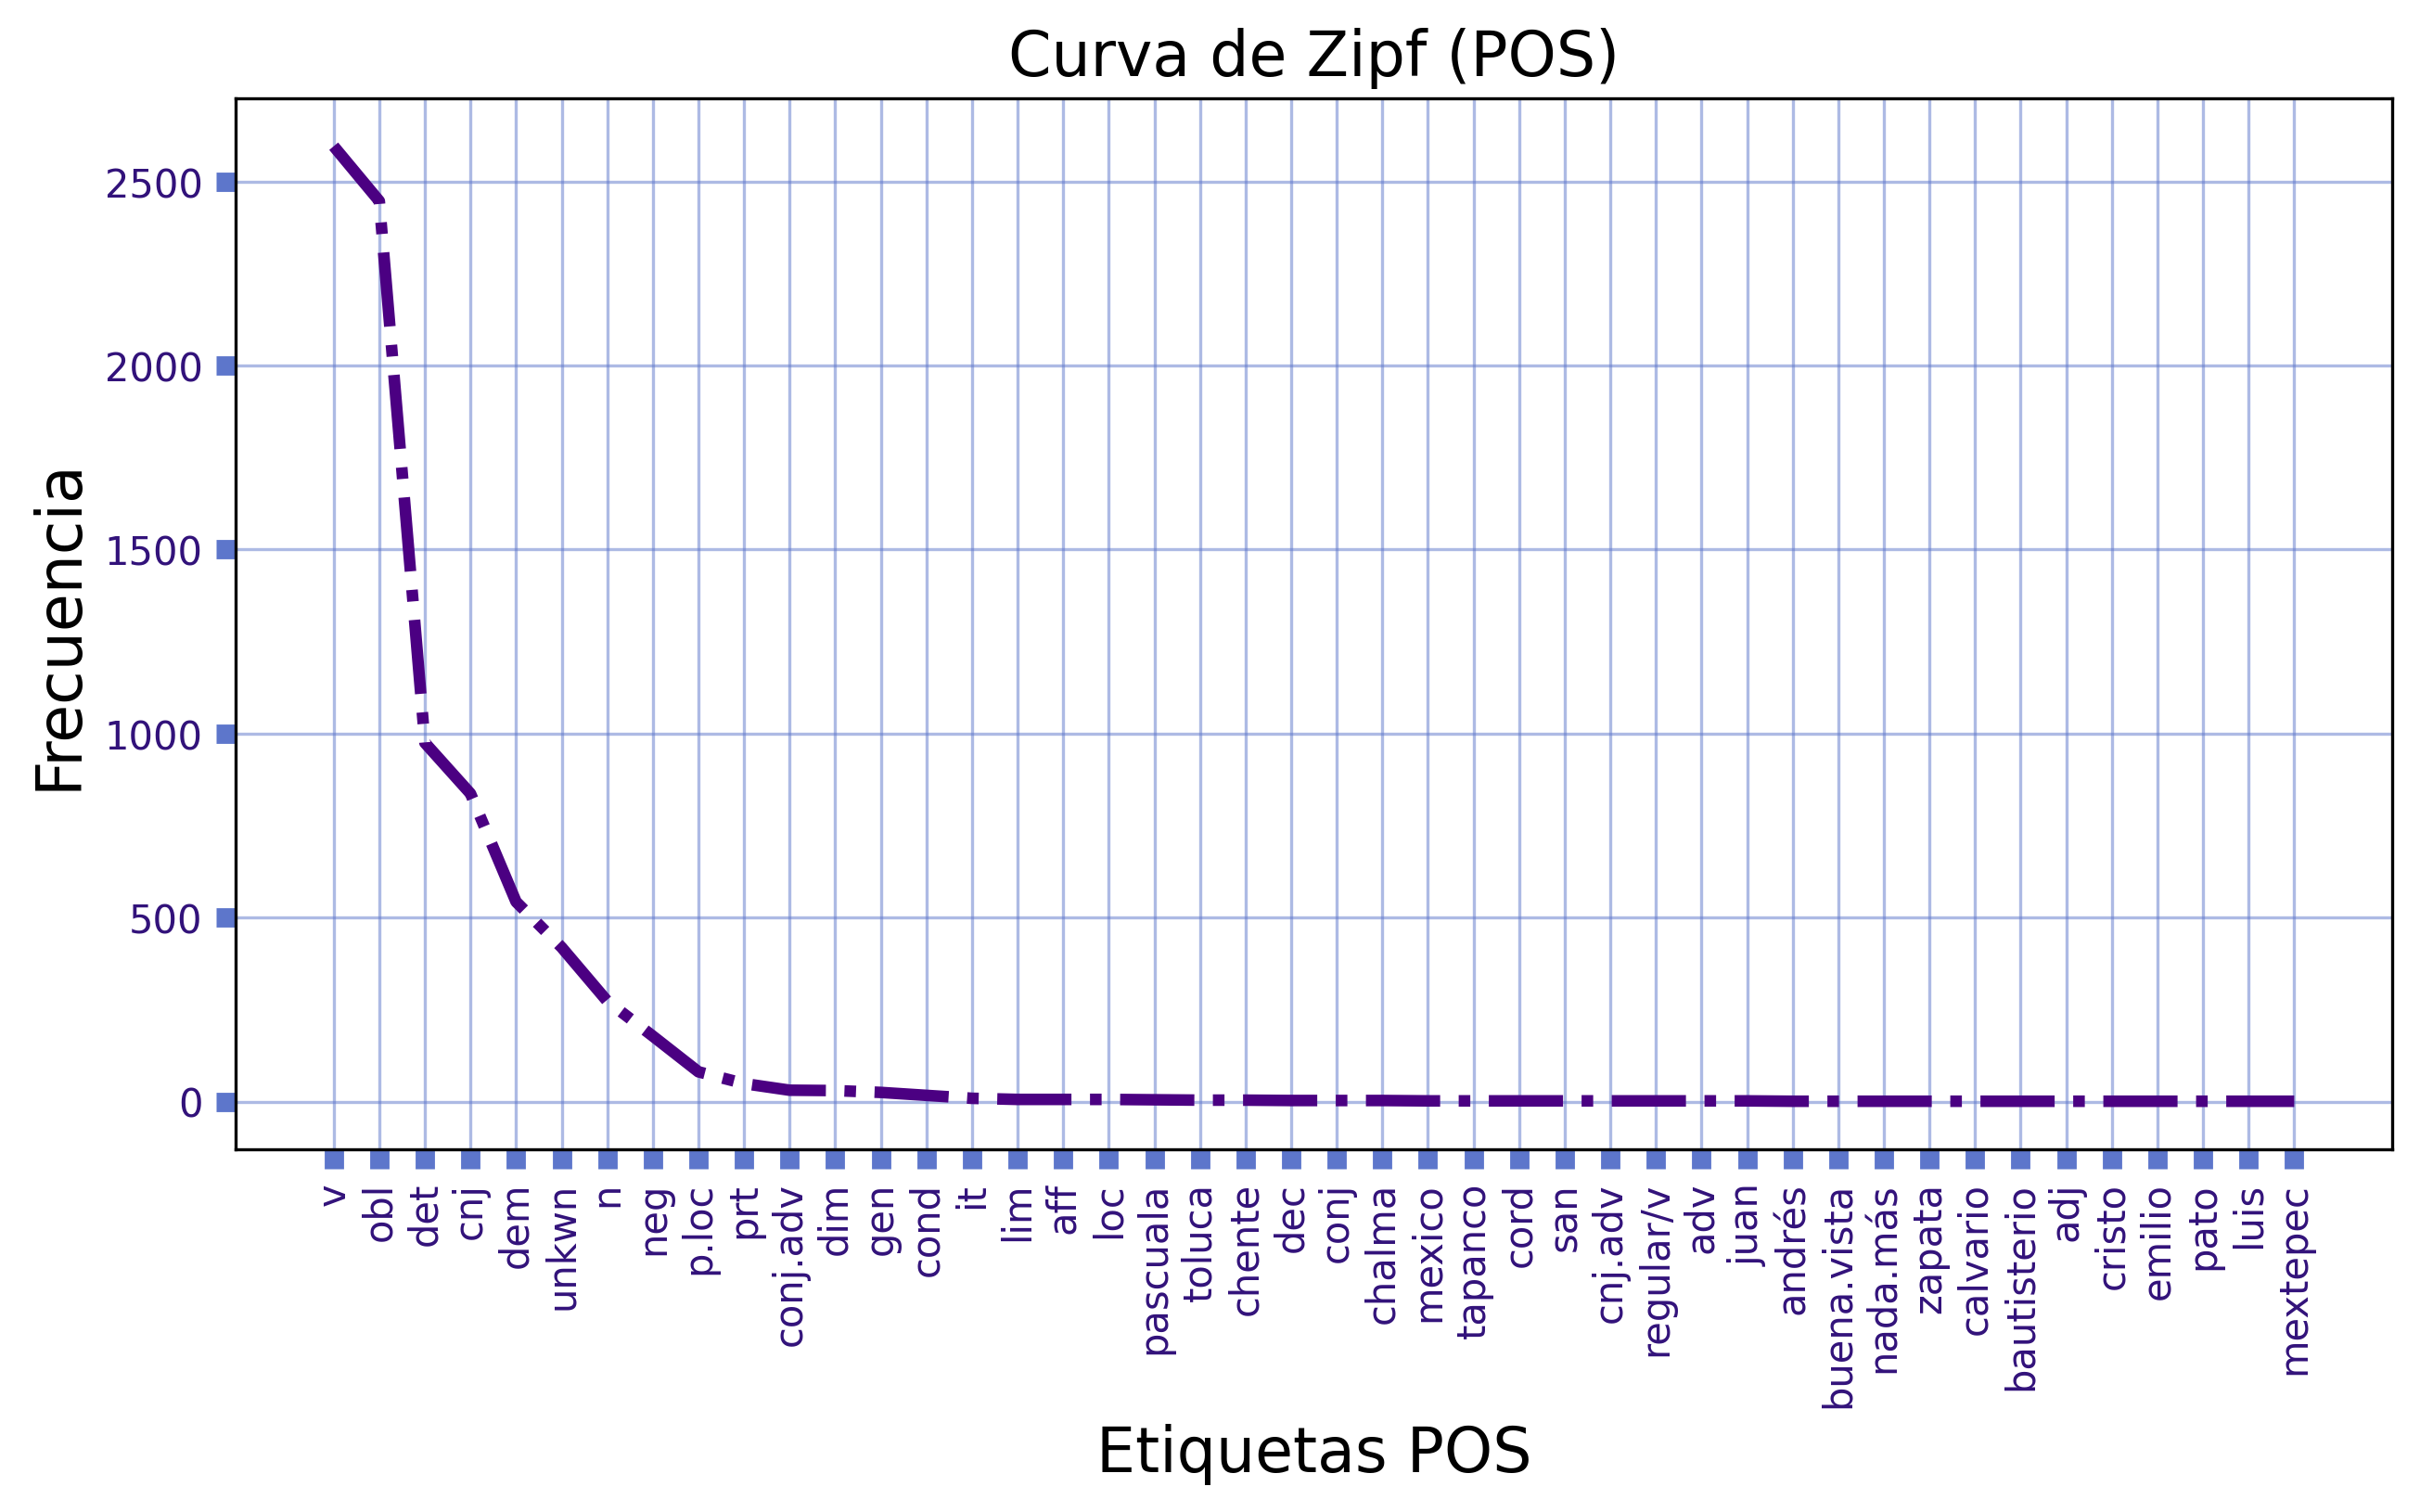
\includegraphics[width=\textwidth]{zipf_pos}
	\caption{Distribución de etiquetas POS}%\Vic{En escala logaritmica}
	\label{fig:pos_distrib}
\end{figure}

Para las etiquetas de Glosa nos basamos en las reglas de \citet{comrie2008leipzig} desarrolladas por el departamento de lingüística del Instituto Max Planck y el Departamento de lingüística de la Universidad de Leipzig. El estándar consiste en diez reglas para la sintaxis y la semántica de glosas interlineales. y un apéndice con un lexicón propuesto de etiquetas de categorías abreviadas \citep{comrie2008leipzig}. Si bien las reglas cubren parte de las necesidades lingüísticas en el glosado de textos, también, son flexibles y se pueden agregar o modificar las convenciones dependiendo de las necesidades.

Los tipos de etiquetas de glosa presentes en el corpus se encuentran en la tabla \ref{table:gloss_types}. En algunos casos aparecen números al inicio de etiquetas que significan las personas gramaticales. Existen combinaciones de varias etiquetas que son separadas por puntos. Por ejemplo, \textsc{pl.exc} es una combinación de las etiquetas ``plural'' y ``exclusivo''.

\begin{table}
	\centering
	\begin{tabular}{| c | c | c | c | c |}\hline
		 stem & det & 3.cpl & psd & lim \\
         prag & 3.icp & lig & det.pl & 1.icp \\
         3.pot & ctrf & 1.pot & pl.exc & 1.cpl \\
         dem & 1.pss & dim & pl & 1.obj \\
         ila & 2.icp & 1.prf & 3.cnt & 3.obj \\
         loc & mod & 1.cnt & 3.pls & prt \\
         it & dual.exc & 3.prf & 3.icp.irr & 3.pss \\
         2.pss & 1.enf & med & dual & p.loc \\
         2.cnt & 2 & 3.imp & int & neg \\
         1.icp.irr & 1.cpl.irr & 2.obj & aum & 1.pls \\
         2.cpl & 2.prf & gen & com & 2.pot\\
         adj & cond  & 3.cpl.irr & 1.sg & encl \\
         3.sg & 3.pss.pl & spt & 1.irr & 2.enf \\
         conj.adv & caus & con & chico & eh \\
         comp & prf & dist mov & 3.irr & det.dem\\
         dcl & nom & 2.icp.irr & & \\
		\hline
	\end{tabular}
	\caption{Glosa}
	\label{table:gloss_types}
\end{table}


El significado para cada etiqueta de glosa se muestra en la tabla \ref{table:gloss_desc}. En esta tabla se omitieron las variaciones de etiquetas con personas gramaticales para compactarla. Además, la distribución de las etiquetas presentes en el corpus se muestran en la figura \ref{fig:gloss_distrib}. Igual que en la figura \ref{fig:pos_distrib} se observa una carga pronunciada en la distribución hacia pocas etiquetas como \textsf{stem}. Este fenómeno es propiciado, en parte, a que son escasos los textos digitales disponibles para el idioma otomí.

\begin{table}
	\centering
	\begin{tabular}{| c  c | c  c |} \hline
		\textbf{Glosa} & \textbf{Significado} & \textbf{Glosa} & \textbf{Significado}\\\hline
		stem & base & ctrf & contrafactual \\
        cpl & completivo & dem & demostrativo \\
        icp & incompletivo & dim & diminutivo \\
        pot & potencial & ila & ilativo \\
        ctn & continuativo & mod & modo \\
        prf & perfecto & loc & locativo \\
        pls & pluscuamperfecto & prt & partícula \\
        irr & irrealis & it & iterativo \\
        imp & imperativo & enf & enfático \\
        psd & pasado & neg & negativo \\
        pl & plural & int & interrogativo \\
        sg & singular & aum & aumentativo \\
        ex & exclusivo & gen & genitivo \\
        pss & posesivo & com & comitativo \\
        obj & objeto & adj & adjetivo \\
        med & voz media & encl & enclítico \\
        dual & número dual & enf & enfático \\
        det & determinante & caus & causativo \\
        lim & limitativo & comp & comparativo \\
        lig & ligadura & dcl & declarativo \\
        prag & partícula pragmática & \\ \hline
	\end{tabular}
	\caption{Descripción de Glosa}
	\label{table:gloss_desc}
\end{table}
	

\begin{figure}
	\centering
	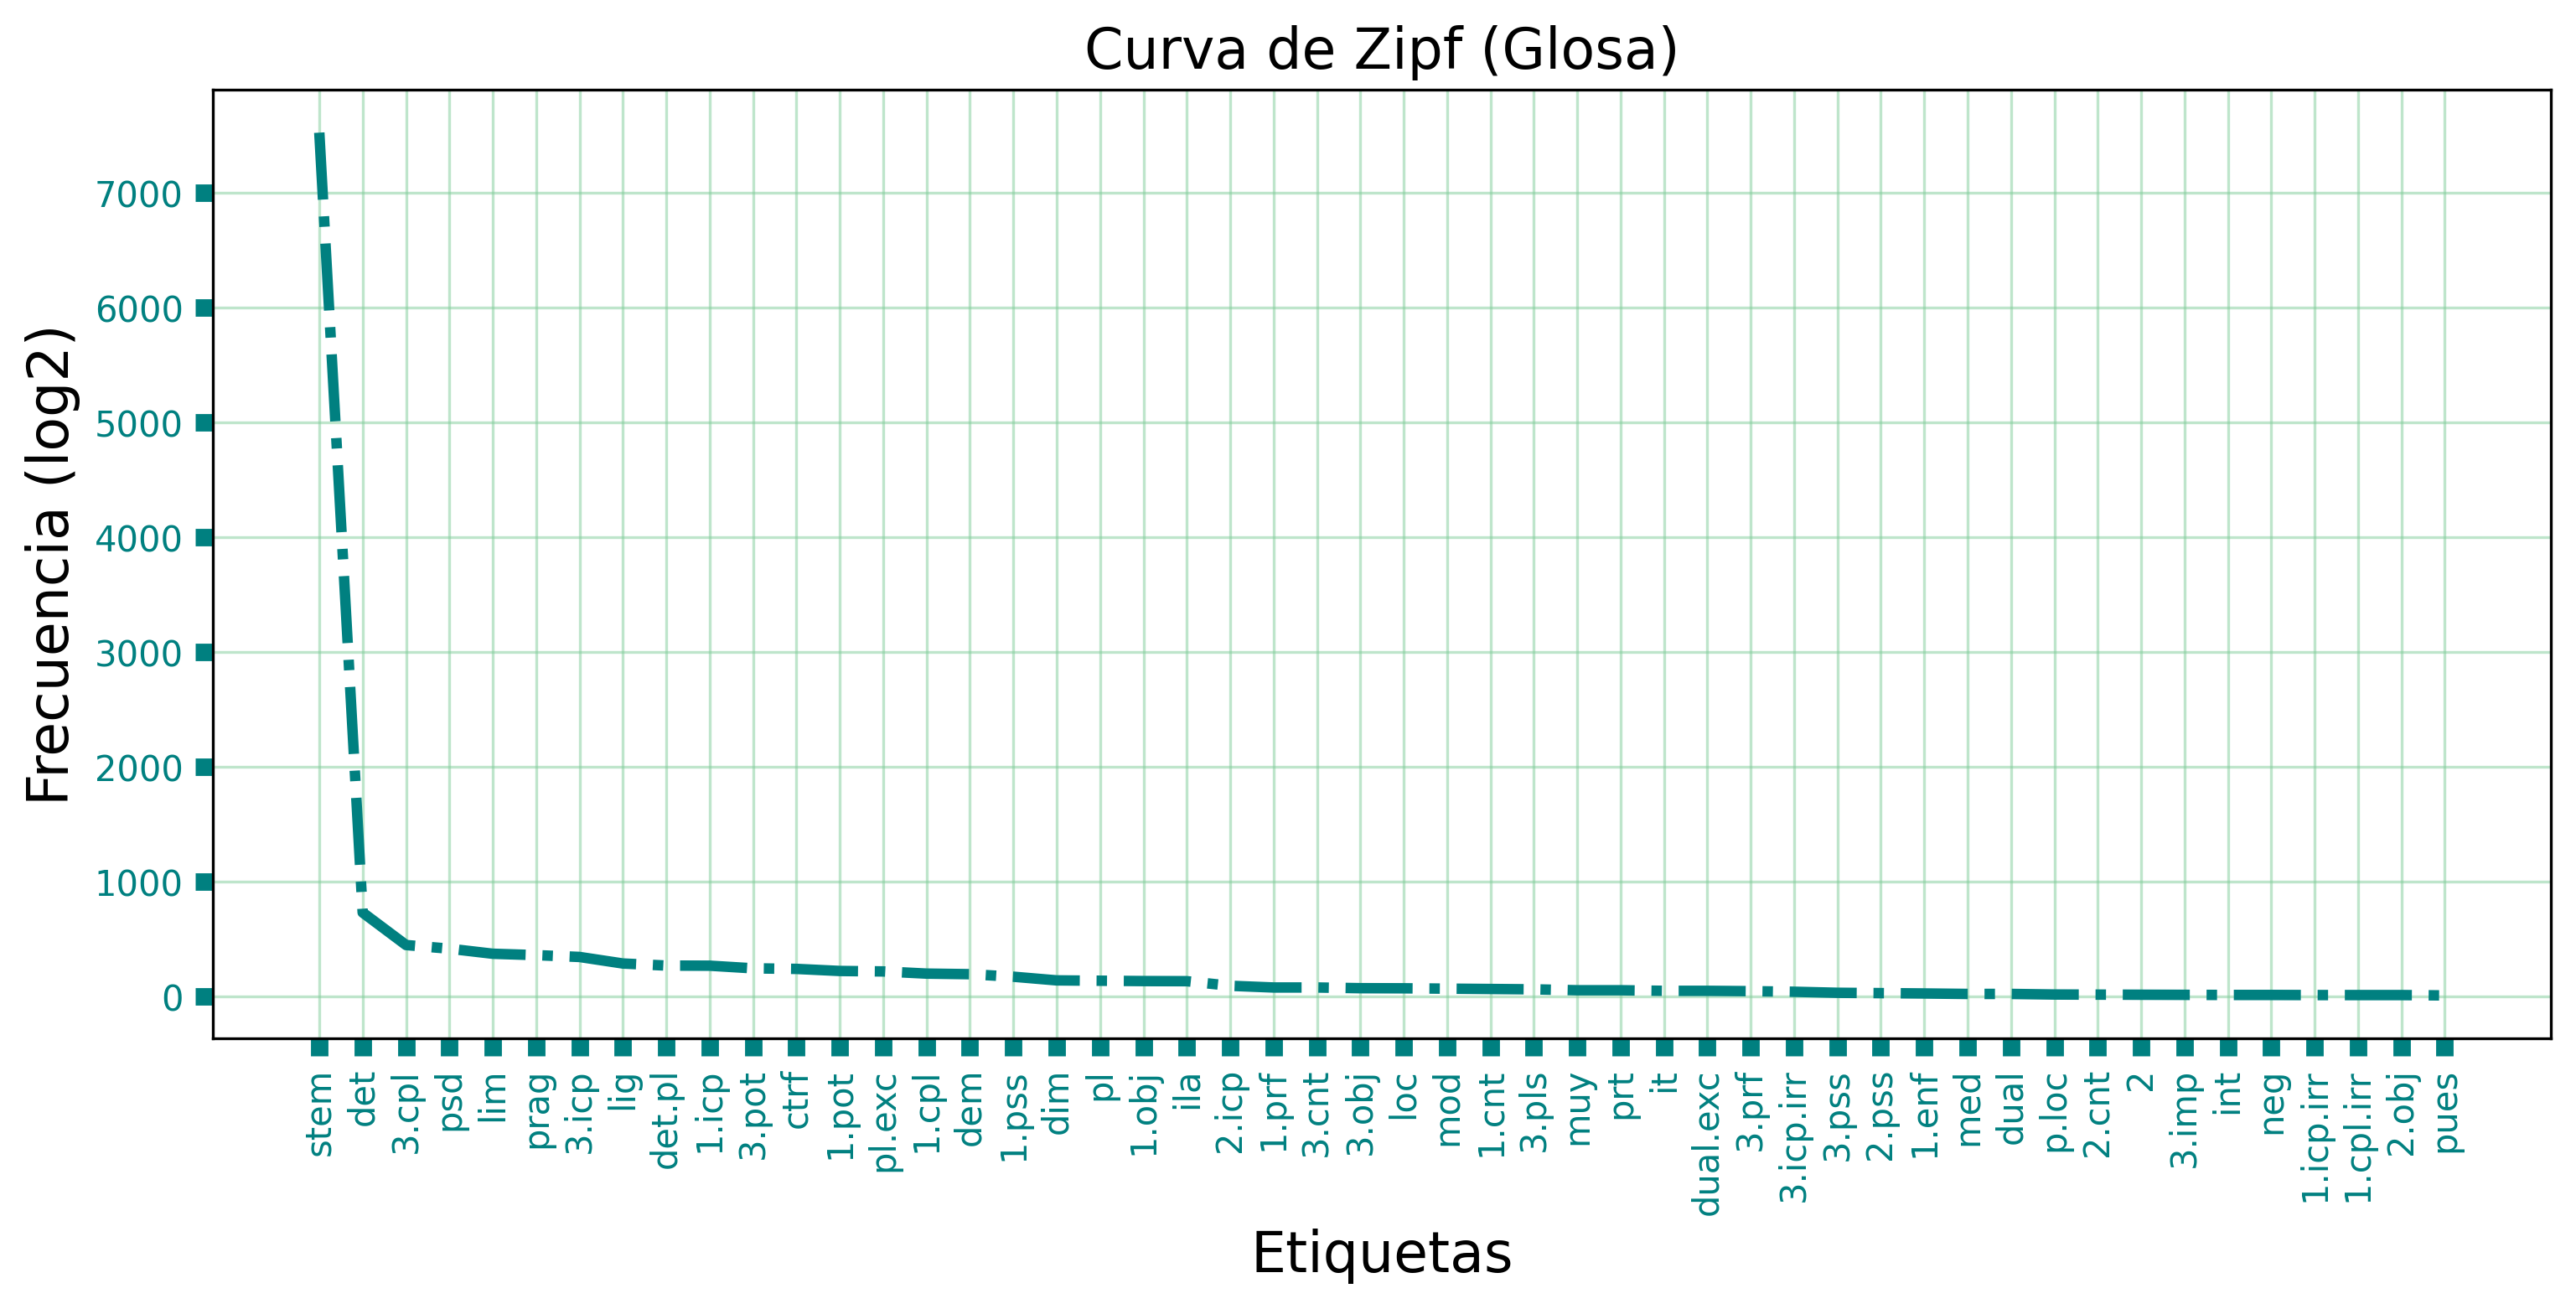
\includegraphics[width=\textwidth]{zipf_gloss}
	\caption{Distribución de glosa (primeras 50)}
	\label{fig:gloss_distrib}
\end{figure}

En las tablas \ref{table_pos_gloss_tokens} se muestran las cuentas de los diez tokens más comunes para las etiquetas \textit{POS} y para la glosa presentes en el corpus. Es destacable tanto la cantidad de oraciones etiquetadas, presentadas en la tabla \ref{table:corpus_length:1}, como la cantidad de tokens de la tabla \ref{table_pos_gloss_tokens} ya que representan un conjunto de textos ínfimo en comparación con los corpus utilizados en métodos de \textit{NLP} convencionales, donde, en general, su desempeño es altamente dependiente de grandes cantidades de textos.

Esta escasez en el corpus es consecuencia de que el idioma otomí es una lengua con bajos recursos digitales. Como menciona \citet{vasquesextraccion} estas lenguas son aquellas que tienen una cantidad limitada de recursos digitales a consecuencia de una baja densidad de hablantes, cuestiones relacionadas con la brecha digital o motivos de otra índole. Gran parte de los métodos tradicionales de \textit{NLP} tienen dificultades importantes para trabajar en entornos de bajos recursos.

\begin{table}[h]
	\centering
	\begin{tabular}{|c | c|}\hline
		\textbf{Etiqueta \textit{POS}} & \textbf{Tokens} \\ \hline
		v & 2579 \\
        obl & 2443 \\
        det & 973 \\
        cnj & 835 \\
        dem & 543 \\
        unkwn & 419 \\
        n & 272 \\
        neg & 176 \\
        p.loc & 81 \\
        prt & 49 \\\hline
	\end{tabular}
	\quad
	\begin{tabular}{|c | c|}\hline                            
		\textbf{Glosa} & \textbf{Tokens} \\ \hline
		stem & 7501 \\
        det & 733 \\
        3.cpl & 444 \\
        psd & 413 \\
        lim & 370 \\
        prag & 357 \\
        3.icp & 341 \\
        lig & 287 \\
        1.icp & 270 \\
        det.pl & 269 \\\hline
	\end{tabular}
	\caption{Tokens de etiquetas (Primeras 10)}
	\label{table_pos_gloss_tokens}
\end{table}

Sin embargo, existen métodos que buscan solucionar el problema de los bajos recursos digitales. Los trabajos de \citet{moeller2018automatic} y \citet{anastasopoulos2018partofspeech}, en particular los \textit{CRFs}, tienen buen desempeño en estas condiciones experimentales.

Esto puede deberse a que los \textit{CRFs}, a diferencia de otros modelos gráficos, toman las virtudes de los modelos generativos y de los modelos condicionales evitando, a su vez, el problema del \textit{bias} que \citet{lafferty2001conditional} define como ``el momento en el cual las transiciones que salen de un estado sólo compiten entre sí, y no con todas las demás transiciones''.

\section{Arquitectura}

% Definir el método en función del marco teórico
% Diagrama de la arquitectura
% Feature functions
% Como se decidieron
% ¿Porque estas caracteristicas son reelevantes?
% Que es para nosotrxs una FF
% Experimentos quitando features functions
% Diagram de donde se encuentran estos elementos en la arquitectura
% Como se calculan lambdas y mu
% Variacion de hiperparámetros
% Descripcion de que variaciones se hicieron
% Hablar de L1 y L2 con ciertas combinaciones
% Mostrar el base line y compararlo
% Metodo de regularizacion y optimización
% Mencionar que se usará un base line
% ¿Cómo se hizo lo que se hizo?
% Preprocesamiento del corpus

Para esta tesis proponemos una arquitectura de aprendizaje estructurado y supervisado utilizando el método gráfico \textit{Conditional Random Fields (CRF)} que permitirá la predicción de secuencias que describen las unidades morfológicas (glosa) dentro de una palabra en otomí. Ya que el resultado esperado es la generación de etiquetas \textit{BIO} que, en principio, son secuenciales, un método que construye el modelo de aprendizaje basándose en gráficas nos pareció adecuado.

Una vez obtenido el corpus, previamente glosado, realizamos una etapa de preprocesamiento del corpus, luego de esta etapa fueron creadas las \textit{feature functions}, que definimos como $X$. Tales funciones contienen información sobre la estructura de la lengua y permiten que la máquina aprenda un modelo para etiquetar secuencias. Cabe señalar que $X$ contiene las \textit{feature functions} que son las entrada de los \textit{CRFs}.

% Previamente debe estar explicado que X son vectores
Debido al enfoque de aprendizaje automático que estamos utilizando consideramos dos conjuntos; un conjunto de entrenamiento y otro de pruebas. Los conjuntos de entrenamiento y pruebas fueron obtenidos del corpus que fue previamente glosados a mano por un experto lingüista.

La etapa de pruebas consistió en aplicar el modelo de aprendizaje al conjunto de evaluación. En ese sentido, aplicar el modelo se refiere a que con el modelo se generaron etiquetas \textit{BIO} para textos del conjunto de pruebas. Con las etiquetas generadas y en comparación con las etiquetas reales se obtuvieron, entre otras medidas de rendimiento, el \textit{accuracy} del modelo. Las secuencias de etiquetas o salidas generadas por el modelo, dadas las observaciones de $X$, fueron definidas como $Y$.

En general, el glosado se realiza manualmente y requiere del expertiz de un lingüista y una cercana cooperación con hablantes nativos quienes reciben capacitación elemental en lingüística y software \citep{moeller2018automatic}. Estas condiciones convierten al glosado manual en una tarea altamente costosa en tiempo y recursos. El objetivo de esta arquitectura es realizar un correcto etiquetado automático de glosa para la lengua otomí, en particular la variante del otomí de Toluca, utilizando técnicas de aprendizaje estructurado y supervisado. Con ello se pretende asistir a personas especializadas, como lingüistas, en el glosado manual.   

Parte de la definición de la estructura de la lengua se encuentra codificada en el conjunto de \textit{feature functions}. Estas funciones describen características de la lengua considerando, detalladamente, el contexto, la posición y etiquetas gramaticales que brindan información útil para la fase de entrenamiento.

Puntualmente, se utiliza un modelo del tipo \textbf{Markov CRF de primer orden con \textit{features} de estado y de transición}. Adicionalmente, fue utilizado el algoritmo de aprendizaje \textbf{Limited-memory Broyden-Fletcher-Goldfarb-Shanno (L-BFGS)}. El algoritmo busca maximizar el logaritmo de probabilidad. Para mejorar el rendimiento son utilizados y modificados un conjunto hiperparámetros.

Estos hiperparámetros son los coeficientes de regularización L1 y L2 necesarios para evitar posible \textit{overfitting}, el número máximo de iteraciones, el número máximo de memorias utilizadas para aproximar la matriz hessiana inversa, epsilon que determina la condición de convergencia, el número de iteraciones para probar el umbral de detención,  delta que define el umbral de detención de cada iteración, el método de búsqueda de línea usado por el algoritmo L-BFGS y el número máximo de intentos para el algoritmo de línea.
El modelo y el algoritmo de aprendizaje fueron tratados a detalle en la sección \ref{sec:marco}.

La arquitectura propuesta abarca desde la obtención del corpus etiquetado, pasando por el preprocesamiento del mismo, llegando a la creación de las \textit{feature functions}, seguido de la separación de los datos en conjuntos de entrenamiento y pruebas, continuando con la fase de entrenamiento y construcción del modelo de aprendizaje, terminando en la etapa de pruebas compuesta por la generación de etiquetas y posterior comparación con la glosa real. Las subsecciones que componen esta arquitectura son \textbf{codificación y preprocesamiento}, \textbf{implementación de los CRFs} y \textbf{feature functions}. En el siguiente capítulo se abordaran las etapas de generación de glosa y pruebas.

La arquitectura de aprendizaje semi-supervisado para la generación de glosa para el otomí de Toluca se describe a continuación.

\subsection{Codificación y preprocesamiento}

Se obtuvo el corpus de un archivo de texto plano. Cada renglón de este archivo es una oración en otomí con glosa. Además, se tiene una etiqueta \textit{POS} por cada palabra. Las frases están estructuradas en forma de listas que contienen otras listas validas para el lenguaje \code{Python}.

La glosa esta presente por cada fragmento de las posibles palabras en otomí. Ejemplificando, la frase \textit{hi tótsogí} (`No lo he dejado') se representa en el corpus como se muestra en el ejemplo \ref{exmp:frase_glosada}.

\begin{exmp} \label{exmp:frase_glosada}
    \textsf{[[[`hi', `stem'], `neg'],
    [[`tó', `1.prf'],
    [`tsogí', `stem'], `v']]}
\end{exmp}

Por último, la lengua otomí tiene una vasta variedad interna lo cual implica diferentes ortografías dependiendo de la región. Tomar en cuenta esta variación ortográfica es de suma importancia para el preprocesamiento. Como menciona \cite{elotl2019otomiprepro} todas las lenguas otomíes son tonales y distinguen entre vocales orales y vocales nasales, existen fonemas que pueden presentarse en unas variantes, mientras que en otras están ausentes. En general, las vocales orales incluyen a las mismas vocales que también se presentan en el español: a, e, i, o, u; pero su inventario de vocales orales no se limita a estas cinco.

\begin{table}[ht]
    \centering
    \begin{tabular}{|c c c c c c|}\hline
        IPA & \textipa{1} & \textipa{E} & \textipa{O} & \textipa{2} & \textipa{9} \\ \hline
        Ortografía práctica & {\b{u}} & {\b{e}} & {\b{a}} & {\b{i}} & {\b{o}} \\
        Convención para este trabajo & $\mu$ & $\epsilon$ & $\alpha$ & $\iota$ & \\ \hline
    \end{tabular}
    \caption{Representación de cada vocal en IPA (alfabeto fonético internacional)}
    \label{tab:vocales_otomi}
\end{table}{}

Ya que el otomí presenta una amplia variedad de vocales, como se puede ver en la tabla, su representación digital puede suponer un reto por la falta de normalización o por la codificación. En nuestro caso, cuando se codificaban algunas vocales para ser representadas como cadenas eran separadas por el lenguaje de programación ocasionando un etiquetando de caracteres que por si solos no tiene sentido. Entonces, fue necesario modificar algunas de las vocales del otomí. Las equivalencias de tales modificaciones pueden observarse en la tabla \ref{tab:vocales_otomi}

Entonces, la estructura de las listas, por renglón, tiene la estructura \code{[[[letras, glosa], [letras, glosa], ..., POS],...]}. Una vez que se obtuvo el corpus de entrenamiento se le aplicó preprocesamiento. El preprocesamiento consistió en asociar, a cada letra de cada palabra, dos elementos; la etiqueta \textit{POS} y una \textit{Bio Label} correspondiente a esa letra.

Retomando el ejemplo \ref{exmp:frase_glosada} y después de aplicar el preprocesamiento el resultado sería el que se muestra en el ejemplo \ref{exmp:frase_preproc}. Cabe señalar que las \textit{BIO-Labels} asignadas dependieron de la posición de la letra como se explico en la sección \ref{sec:marco}.

\begin{exmp} \label{exmp:frase_preproc}
    \textsf{[[['h', 'neg', 'B-stem'], ['i', 'neg', 'I-stem']], [['t', 'v', 'B-1.prf'],
          ['ó', 'v', 'I-1.prf'],
          ['t', 'v', 'B-stem'],
          ['s', 'v', 'I-stem'],
          ['o', 'v', 'I-stem'],
          ['g', 'v', 'I-stem'],
          ['í', 'v', 'I-stem']]]}
\end{exmp}

Con las palabras etiquetadas a nivel de letra se obtuvo un conjunto de entrenamiento y un conjunto de pruebas. Por una parte, el conjunto de entrenamiento permitió la observación de ejemplos y la posterior generación de un modelo de aprendizaje. Por otro lado, con el conjunto de pruebas obtuvimos el \textit{accuracy} del modelos etiquetando frases no vistas. Es importante destacar que estos dos conjuntos estuvieron completamente separados ya que mezclar el conjunto de entrenamiento y de pruebas pudo habernos llevado a resultados erroneos y sesgados.

Previo al entrenamiento se construyeron las \textit{feature functions} con el conjunto de entrenamiento. En ese sentido, por cada letra etiquetada de las palabras en otomí se tuvo una \textit{feature function} y por cada \textit{feature function} se tiene una \textit{Bio Label} asociada. La construcción de estas funciones será descrita a profundidad en la subsección \ref{subsec:feature}.

% Entrenamiento

Los \textit{CRFs} recibieron como entrada las \textit{feature functions}, representadas por un vector $X$ y sus respectivas \textit{Bio Labels}, representadas por un vector $y$, asociadas con cada \textit{feature function} con concordancia uno a uno respetando la posición. 

% Feature functions
\subsection{Feature functions} \label{subsec:feature}

La extracción de estas características es importante porque capturar fenómenos lingüísticos necesarios para que la estructura de la lengua se pueda plasmar en el modelo de aprendizaje. Estas características están capturando, entres otras cosas, el contexto de la palabra y es importante para predecir la morfología. Para construir las \textit{feature functions} se necesita el corpus glosado y etiquetado a nivel de letra. Se extrajeron las siguientes características para cada letra en el corpus:

\begin{description} \label{feature_functions_descr}
    \item[Bias:] Esta característica captura la proporción de una etiqueta dada en el conjunto de entrenamiento. El modelo aprende los pesos asociados con las etiquetas como si las etiquetas se generaran independientemente de una distribución de probabilidad dada. Ayuda a tomar en cuenta que algunas etiquetas son poco usuales y otras muy usuales.
    
    \item[\textsf{letterLowercase}:] Toma la letra y la convierte a minúsculas. Es importante para la creación del modelo tener en cuenta la letra que se esta viendo en un momento determinado para las predicciones posteriores. 
    
    \item[\textsf{prevpostag} y \textsf{nxtpostag}:] Es conveniente y muy útil tomar en cuenta las etiquetas \textit{POS} ya que brindan información gramatical de la palabra que se observa en ese momento. Tal información se basa en la morfología y algunas veces en la sintaxis de la lengua.

    \textsf{prevpostag} toma la etiqueta POS previa (Si existe) y \textsf{nxtpostag} toma la etiqueta POS siguiente (Si existe)
    
    \item[\textsf{BOS}, \textsf{EOS}, \textsf{BOW} y \textsf{EOW}:] Indicar el inicio y fin de frase y palabras otorga la capacidad de ver que tipo de palabras se está viendo en ese momento. Por ejemplo, transiciones que propician estados iniciales y finales brindan información contextual.

    \textsf{BOS} indica el inicio de la frase, \textsf{EOS} indica el fin de la frase \textsf{BOW} indica el inicio de la palabra y \textsf{EOW} indica el final de la palabra.
    
    \item[\textsf{letterposition}:] Indica la posición de la letra en la palabra. Otorga más información sobre el contexto de la palabra en la frase que se observa en un determinado momento.
    
    \item[\textsf{prev<n>letters} y \textsf{nxt<n>letters}:] La recuperación de ventanas de contexto son convenientes para del otomí ya que se trata de una lengua aglutinante dónde, en general, las palabras son largas. En particular, la longitud promedio de las palabras en el corpus es de 4.89\footnote{Promedio de la distribución de palabras basada en  en tokens. Para una distribución por tipos se obtuvo 7.2}. Esta característica da la pauta para que la observación del contexto en un determinado momento sea relevante para la construcción del modelo.
    
    \textsf{prev<n>letters} toma las $n$ letras previas y \textsf{nxt<n>letters} toma las $n$ letras siguientes, si existen en ambos casos. La variable $n$ determina el nombre de la \textit{feature} que indica el tamaño de la ventana a partir de la letra que se esta viendo en ese momento y va desde el número uno, caso dónde no se incluye número en el nombre, hasta el número cuatro. Por ejemplo, \textsf{prev4letters} toma las cuatro letras previas y \textsf{nxtletter} toma la letra siguiente.

\end{description}

Las características mencionadas son información relevante para poder construir un modelo más preciso dadas las estructuras de la lengua. Dichas características pueden o no estar presentes dependiendo de la letra que se esté viendo en ese momento. Por ejemplo, si es la primer letra de una palabra la que se observa no estarán presentes las características \textsf{prevletter}, \textsf{prev2letters} o \textsf{EOW} por mencionar algunas. Características como \textsf{letterLowercase} o \textsf{bias} siempre estuvieron presentes.

La construcción de las \textit{feature functions} dependió del experimento en turno. Por ejemplo, en algunos casos fueron modificadas reduciéndolas ignorando las etiquetas que brindaban información gramatical o fueron construidas para solo observar la letra actual y la anterior simulando un \textit{Hidden Markov Model (HMM)} utilizando \textit{CRFs}.

% hiperparámetros
\subsection{Implementación de CRFs y entrenamiento}

El termino \textit{CRFs} se refiere a una familia de métodos de aprendizaje basados en gráficas. En concreto, para la generación de secuencias de etiquetas utilizamos \textit{linear-chain CRF}. Este método requiere de un algoritmo de optimización. Como ya mencionamos previamente utilizamos el \textit{L-BFGS}. Este algoritmo mejora los pesos de las funciones muy lentamente al comienzo de un proceso de entrenamiento, pero al final converge rápidamente en los pesos óptimos de las funciones.

El entrenamiento consistió en la búsqueda de un modelo que maximiza el logaritmo de verosimilitud con el método de aprendizaje \textit{L-BFGS}. Es necesario entonces definir los parámetros del algoritmo de maximización. Los hiperparámetros modificados fueron los de \textit{Elastic Net} con valores de regularización L1 + L2. También, fue configurado el número máximo de iteraciones para el algoritmo pero fue fijado en $50$ para todos los modelos. El resto de hiperparámetros se dejaron con un valor predeterminado. En la tabla \ref{tab:hyper_default_values} se muestran los valores que no se modificaron para los hiperparámetros.

\begin{table}[]
    \centering
    \begin{tabular}{| c | c |}\hline
        \textbf{Hiperparámetro} & Valor \\\hline
        \textsf{max\_iterarions} & 50 \\
        \textsf{num\_memories} & 6 \\
        \textsf{epsilon} & $1*10^{-5}$ \\
        \textsf{stop} & 10 \\
        \textsf{delta} & $1*10^{-5}$ \\
        \textsf{linesearch} & ``MoreThuente'' \\
        \textsf{max\_linesearch} & 20 \\\hline
    \end{tabular}
    \caption{Valores de los hiperparámetros}
    \label{tab:hyper_default_values}
\end{table}

Además de los hiperparámetros se configuraron diferentes entornos de experimentación dónde se construyeron \textit{feature functions} con mas o menos información. En la tabla \ref{tab:models-config} se listan las diferentes configuraciones implementadas en esta tesis.

% Modelos

\begin{table}[ht]
    \centering
    \begin{tabular}{| c | c | c | c | c |}\hline
        \textbf{Modelo} & \textbf{L1} & \textbf{L2} & \textbf{Features}\\ \hline
        \textsf{linearCRF\_l2\_zero} & 0.1 & 0 & Todas las disponibles\\
        \textsf{linearCRF\_featured} & 0.1 & $1*10^{-3}$ & Todas las disponibles\\
        \textsf{linearCRF\_l1\_l2\_zero} & 0 & 0 & Todas las disponibles\\
        \textsf{POS\_Less} & 0.1 & $1*10^{-3}$ & Sin etiquetas \textit{POS}\\
        \textsf{linearCRF\_l1\_zero} & 0 & $1*10^{-3}$ & Todas las disponibles\\
        \textsf{POS\_Less\_l1\_zero} & 0 & $1*10^{-3}$ & Sin etiquetas \textit{POS}\\
        \textsf{POS\_Less\_l1\_l2\_zero} & 0 & 0 & Sin etiquetas \textit{POS}\\
        \textsf{HMMLike\_l2\_zero} & 0.1 & 0 & Mínimas\\
        \textsf{HMMLike\_regularization} & 0.1 & $1*10^{-3}$ & Mínimas\\\rowcolor{Yellow}
        \textsf{baseline\_HMMLike\_zero} & 0 & 0 & Mínimas\\
        \textsf{HMMLike\_l1\_zero} & 0 & $1*10^{-3}$ & Mínimas\\\hline
    \end{tabular}
    \caption{Modelos de aprendizaje}
    \label{tab:models-config}
\end{table}

% Testing
Terminada la fase de entrenamiento y construido el modelo de aprendizaje se puso a prueba con el conjunto destinado a este propósito y que fue previamente obtenido. Similar a la fase de entrenamiento las entradas fueron las \textit{feature functions} y la \textit{Bio Labels} asociada a cada \textit{feature function}. Utilizando el modelo de aprendizaje se etiquetó cada letra con base en la estructura de la lengua codificada en las \textit{feature functions}. Las etiquetas generadas fueron comparadas con las reales y con ello se obtuvo la exactitud del modelo. 

Recapitulando, se obtuvo un corpus en otomí previamente glosado por un experto lingüista, después, en la etapa de codificación estructuramos la información de la lengua y en el preprocesamiento se crearon las \textit{feature functions} que serán las entradas de los \textit{CRFs}, continuamos con la fase de entrenamiento, creación del modelo de aprendizaje. Por último, se ejecuto la fase de evaluación comparando las \textit{BIO-Labels} generadas por el modelo y las reales presentes en el conjunto de pruebas recuperando el \textit{accuracy} del modelo. La arquitectura final se puede observar en la figura \ref{fig:architecture}.

\begin{figure}[ht]
	\centering
	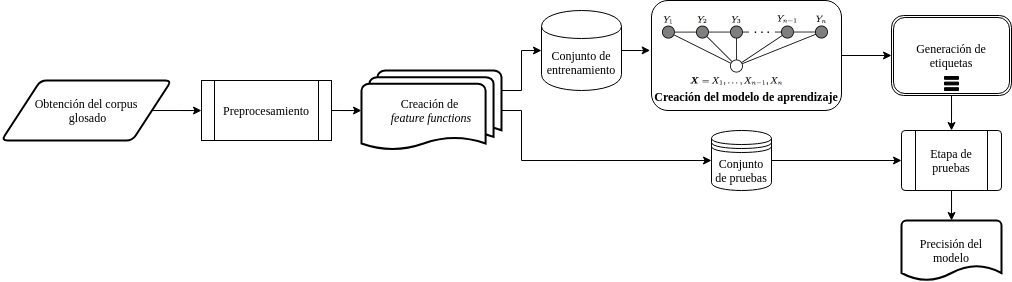
\includegraphics[width=\textwidth]{img/arquitectura}
	\caption{Arquitectura de aprendizaje}
	\label{fig:architecture}
\end{figure}

\subsubsection{Hardware utilizado}

En la fase de experimentación fue utilizado el paquete \textsf{python-crfsuite} que es un \textit{binding} de la implementación de \citet{CRFsuite} para CRFs para lenguaje de programación \textit{Python} en su versión \textit{3.7}. La fase de experimentación corrió en una maquina con un procesador \textsf{Intel i7-7700HQ @ 3.800GHz} con \textsf{16 GB} de memoria principal. En promedio una corrida de entrenamiento y evaluación \textit{K-folds} con \textit{k=10} tomó 52 minutos.


\chapter{Resultados}
% Solo reportar

En este capítulo se examinará el método de evaluación utilizado para la construcción de los modelos de aprendizaje. Además, se detallará el desempeño de los modelos que fueron mencionados en el capítulo \ref{chap:metodology} y se profundizará en los resultados obtenidos en los diferentes entornos de experimentación. 

% Mostrar la comparación a profundidad del baseline con todos los experimentos
% Demostrar que lo que propusimos fue mejor
% Cualitativos y cuantitativos
% Hablar del Baseline y como mejoró con mas features
% explicar como ayudo la información de las Feature functions
% Definir como plantear la historia: 
    % De lo mas básico (baseline) y ver como lo mejoramos con las feature functions
    % El conocimiento lingüístico ayuda a mejorar

\section{Evaluación}

Propusimos diferentes entornos de experimentación dónde fueron modificadas las \textit{feature functions} y los parámetros de regularización \textit{Elastic Net} L1 + L2. En concreto, se presentaron tres entornos de evaluación; en el primero se redujeron las \textit{features} al mínimo, utilizando la información de la letra actual en la palabra y la letra anterior relativa a la letra actual, con lo que se simulaba un \textit{Hidden Markov Model (HMM)}; en el segundo, se modificaron las \textit{features} para ignorar las etiquetas \textit{POS}, y en el último, se utilizaron todas las \textit{features} disponibles, que se mencionaron en la sección \ref{feature_functions_descr}.

Para comparar el desempeño entre los modelos construidos, presentes en la tabla \ref{tab:models-config}, seleccionamos como base el entorno dónde se simula un \textit{HMM} que corresponde con el modelo \textsf{baseline\_HMMLike\_zero}.

% Pasar a resultados
Para saber que tan buenas son las predicciones de un modelo generado es necesario validar su desempeño. La forma mas sencilla de realizar esta validación es partir el corpus en dos conjuntos; el primer conjunto será destinado al entrenamiento del modelo y el segundo conjunto, independiente del conjunto de entrenamiento, tendrá el propósito de evaluar el desempeño del modelo. Realizar esta partición equivale a dividir aleatoriamente nuestro corpus en dos partes. Está técnica de validación es conocida como \textit{Hold Out}.

Sin embargo, este método de validación supone inconvenientes. Por un lado, es obligatorio sacrificar una parte del corpus para la realización de pruebas y, por otro lado, el desempeño del modelos podría mostrar valores muy optimistas o muy pesimistas dependiendo solo de cómo se realiza la partición del corpus.

% Aquí se habla del K fold
Un método de validación más adecuado para nuestros entornos de experimentación es el de \textit{K-fold cross-validation}. Esta técnica está diseñada para medir el desempeño sin sacrificar muchos datos. 

En \textit{K-fold} el corpus es dividido en $K$ subconjuntos (\textit{folds}) a diferencia de \textit{Hold Out} donde se divide solo en dos partes. Se toma un subconjunto para pruebas y el resto es usado para la etapa de entrenamiento. El modelo es entrenado y después se obtiene el \textit{accuracy} utilizando el subconjunto de pruebas antes mencionado. El \textit{accuracy} es obtenido como se muestra en la ecuación \ref{eq:accuracy}.

\begin{equation}\label{eq:accuracy}
    accuracy = \frac{VP + VN}{VP + VN + FP + FN}
\end{equation}

dónde \textit{VP} es Verdadero Positivo, \textit{VN} es Verdadero Negativo, \textit{FP} es Falso Positivo y \textit{FN} es Falso Negativo.

El proceso se repite $K$ veces hasta que cada subconjunto fue utilizado en la etapa de pruebas. Finalmente, se promedian los $K$ \textit{accuracy} obtenidos en cada prueba para tener el \textit{accuracy} general del modelo que es el que reportamos. En la figura \ref{fig:k-fold} se muestra una representación gráfica del método de evaluación con $K = 5$. Para todas las etapas de entrenamiento-evaluación utilizamos $K = 10$.

Consideramos exitosa la predicción si se logra maximizar la correcta clasificación de las etiquetas de salida.

\begin{figure}[ht]
    \centering
    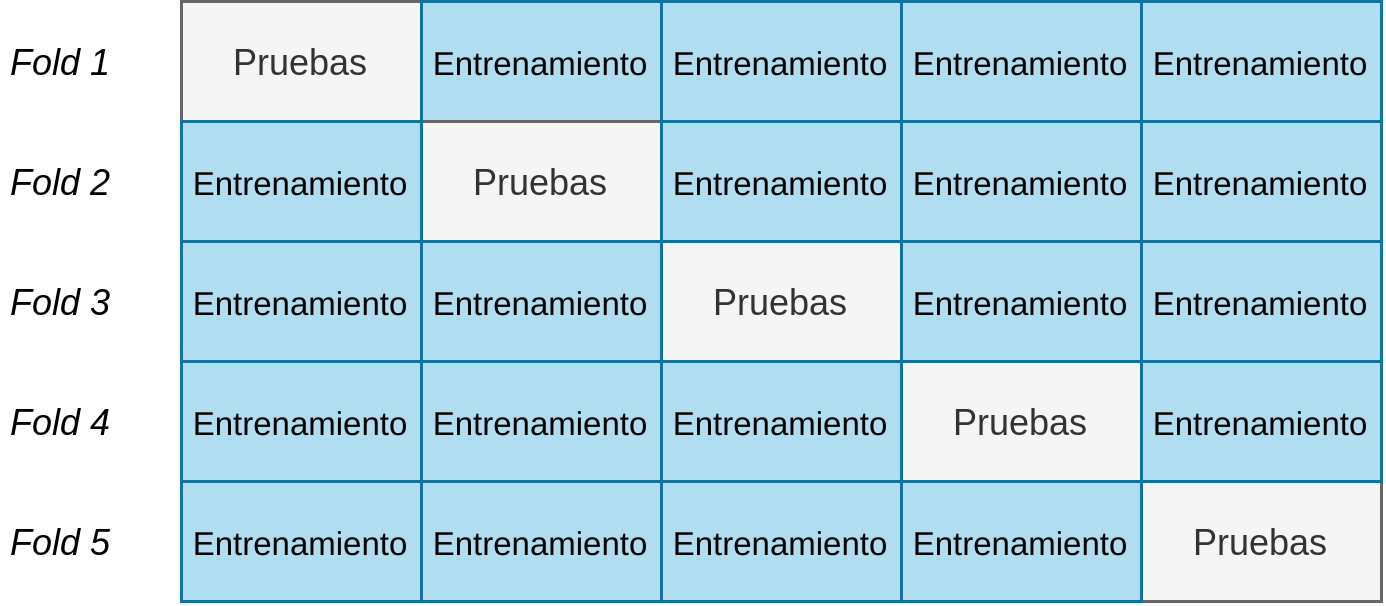
\includegraphics[scale=0.8]{img/kfold.png}
    \caption{Representación gráfica de \textit{K-fold cross-validation}}
    \label{fig:k-fold}
\end{figure}

A continuación mostramos los modelos resultantes de cada etapa de experimentación propuestas en este trabajo.

En la tabla \ref{tab:models-full-featured} se muestran los modelos dónde se recuperaron todas las \textit{features} disponibles. A este entorno de experimentación lo llamaremos \textit{LinearCRF}.\footnote{Tiempos de entrenamiento (minutos): linearCRF\_l2\_zero=41.86, linearCRF\_featured=42.91, linearCRF\_l1\_l2\_zero=39.46, linearCRF\_l1\_zero=41.03}

\begin{table}[ht]
    \centering
    \begin{tabular}{| c | c | c | c |}\hline
    \textbf{Modelo} & \textbf{Accuracy}\\\hline
    \textbf{\textsf{linearCRF\_l2\_zero}} & \textbf{0.9516}\\
    \textsf{linearCRF\_featured} & 0.9509\\
    \textsf{linearCRF\_l1\_l2\_zero} & 0.9499\\
    \textsf{linearCRF\_l1\_zero} & 0.948\\\hline
    \end{tabular}
    \caption{Modelos con todas las \textit{features} disponibles}
    \label{tab:models-full-featured}
\end{table}

En la tabla \ref{tab:models-pos-less} se encuentran los modelos que pertenecen al entorno de experimentación donde fueron ignoradas las etiquetas \textit{POS}. Este entorno de experimentación lo llamaremos \textit{POSLess}.\footnote{Tiempos de entrenamiento (minutos): POS\_Less=37.91, POS\_Less\_l1\_zero=40.25, POS\_Less\_l1\_l2\_zero=36.67}

\begin{table}[ht]
    \centering
    \begin{tabular}{| c | c | c | c |}\hline
    \textbf{Modelo} & \textbf{Accuracy}\\\hline
    \textbf{\textsf{POS\_Less}} & \textbf{0.9499}\\
    \textsf{POS\_Less\_l1\_zero} & 0.9473\\
    \textsf{POS\_Less\_l1\_l2\_zero} & 0.9452\\\hline
    \end{tabular}
    \caption{Modelos donde se ignoran las etiquetas \textit{POS}}
    \label{tab:models-pos-less}
\end{table}

En la tabla \ref{tab:models-hmmlike} se aprecian los modelos generados en el entorno de experimentación con las \textit{feature functions} reducidas al mínimo, simulando \textit{HMMs}. Este entrono de experimentación será llamado \textit{HMMLike}.\footnote{Tiempos de entrenamiento (minutos): HMMLike\_l2\_zero=43.71, HMMLike\_regularization=42.98, baseline\_HMMLike\_zero=40.44, HMMLike\_l1\_zero=43.9 }

\begin{table}[ht]
    \centering
    \begin{tabular}{| c | c | c | c |}\hline
    \textbf{Modelo} & \textbf{Accuracy}\\\hline
    \textbf{\textsf{HMMLike\_l2\_zero}} & \textbf{0.8818}\\
    \textsf{HMMLike\_regularization} & 0.8791\\
    \textsf{baseline\_HMMLike\_zero} & 0.8762\\
    \textsf{HMMLike\_l1\_zero} & 0.8745\\\hline
    \end{tabular}
    \caption{Modelos que simulan \textit{HMMs}}
    \label{tab:models-hmmlike}
\end{table}

\section{Análisis de resultados}

% Hablar de HMM
% cual salio peor
En principio, el entorno de experimentación dónde simulamos \textit{HMMs} y en concreto el modelo \textsf{baseline\_HMMLike\_zero} fue el que tomamos como base para poder comparar el desempeños de los \textit{CRFs}. En la tabla \ref{tab:models-hmmlike} se pueden ver los modelos construidos en este entorno.

Es importante destacar que este entorno de mínima información simula el método de generación de etiquetas \textit{HMM} pero no es, en sentido estricto, un \textit{HMM}\footnote{Una diferencia entre los \textit{HMM} simulados con el modelo gráfico \textit{CRF} y los \textit{HMM} tradicionales radica en que los \textit{CRFs} son grafos no dirigido. Además, los \textit{HMM} son modelos generativo, mientras que los \textit{CRFs} son modelos discriminativos}
\diego{referencia} ya que fueron utilizados los \textit{CRFs} para su construcción.

El modelo con el \textit{accuracy} más bajo se encuentra en este entorno de experimentación y es \textsf{HMMLike\_l1\_zero} con un $87.45\%$ de \textit{accuracy}. Por otra parte, el modelo propuesto como base supera en al modelo \textsf{HMMLike\_l1\_zero} por apenas $1.7*10^{-3}$ unidades. Notamos que variando los hiperparametros $L_1$ y $L_2$ para este entorno de experimentación se obtuvo una mejora de apenas $5.6*10^{-3}$ respecto al modelo base. 

% Hablar de POSLess
Continuando con el segundo entorno de experimentación, dónde se construyó el \textit{linear Chain CRF} ignorando las etiquetas \textit{POS}, el \textit{accuracy} mejoró de forma considerable respecto a los modelos que simulaban \textit{HMMs}. Como se puede ver en la tabla \ref{tab:models-pos-less} todos los modelos de este entorno lograron al menos un \textit{accuracy} del $94\%$. Observamos una mejora poco significativa con la variación de los hiperparametros $L_1$ y $L_2$. En este entorno el modelo con mayor \textit{accuracy} fue \textsf{POS\_Less} con $94.99\%$. 

Por último, el entorno dónde se construyeron los \textit{linear Chain CRFs} tomando todas las \textit{features} disponibles, mencionadas en \ref{feature_functions_descr}, fue en el que se obtuvo el mejor desempeño. Los modelos generados en este entorno obtuvieron entre $94\%$ y $95\%$ de \textit{accuracy}. Una vez más, la variación de hiperparametros de regularización comprobó mejoras leves en los modelos. Destacamos además que la mejora con respecto al entorno de experimentación \textit{POSLess} es de apenas $1\%$ en los modelos con mejor desempeño del entorno \textit{linearCRF}. En la tabla \ref{tab:models-comparation} se muestra la comparación entre el modelo base y los modelos con mejor \textit{accuracy} en los otros entornos de experimentación.

\begin{table}[ht]
    \centering
    \begin{tabular}{| c | c |}\hline
        \textbf{Modelo} & \textbf{Accuracy} \\\hline
        \textbf{\textsf{linearCRF\_l2\_zero}} & \textbf{0.9516}\\ 
        \textsf{POS\_Less} & 0.9499\\ 
        \textsf{baseline\_HMMLike\_zero} & 0.8762\\ \hline
    \end{tabular}
    \caption{Comparación de modelos de diferentes entornos con mejor \textit{accuracy}}
    \label{tab:models-comparation}
\end{table}  

Comparando el rendimiento de los modelos a través de los entornos de experimentación observamos lo siguiente; entornos ricos en información, codificada en las \textit{feature functions}, obtienen un desempeño mayor en comparación con los entornos dónde se disponía de información mínima.

% logramos pasar el base line?
% que features fueron determinantes?
% Cual salio mejor
Con base en la arquitectura propuesta observamos que el modelo  \textbf{\textsf{linearCRF\_l2\_zero}} obtuvo el mejor \textit{accuracy} y que supera el modelo base propuesto \textbf{\textsf{baseline\_HMMLike\_zero}} (Ver tabla \ref{tab:models-comparation}). Del análisis a través de los entornos de experimentación podemos concluir, por un lado, que con la variación de hiperparametros en las tres familias de modelos (\textsf{linearCRF}, \textsf{POS\_Less}, \textsf{HMMLike}) (Ver tablas \ref{tab:models-full-featured}, \ref{tab:models-pos-less}, \ref{tab:models-hmmlike}), se obtuvo una mejora en el \textit{accuracy} poco representativa; por otra parte, el \textit{accuracy} que muestran los modelos \textsf{POS\_Less} y \textsf{linearCRF} es muy similar.

\diego{Modificar y mencionar que las etiquetas POS no son tan importantes}
Entonces, parece ser que la configuración de los hiperparametros \textit{Elastic Net} y las etiquetas \textit{POS} (codificadas en las \textit{feature functions}) mejoran levemente el desempeño de los modelos. Además, podemos concluir que el resto de información de la lengua, codificada también en las \textit{features functions}, es la que determinan, en gran medida, el desempeño de los \textit{CRFs} para la correcta generación de \textit{BIO Labels} (glosa) para el idioma otomí.

Algo destacable es que las etiquetas \textit{POS} no parecen ser tan relevante debido a que existen características morfológicas (patrones presentes en las mismas palabras) o sintácticas (secuencias de palabras) que indican la categoría de la palabra. Por ejemplo, los sustantivos en su mayoría son precedidos de `ri' o `yi' (artículos singular y plural, respectivamente). Asimismo, los verbos tienen una morfología particular y existen patrones que muestran que se trata de un verbo: prefijos flexivos, sufijos, formativos temáticos, etc.

\begin{figure}[ht]
	\centering
	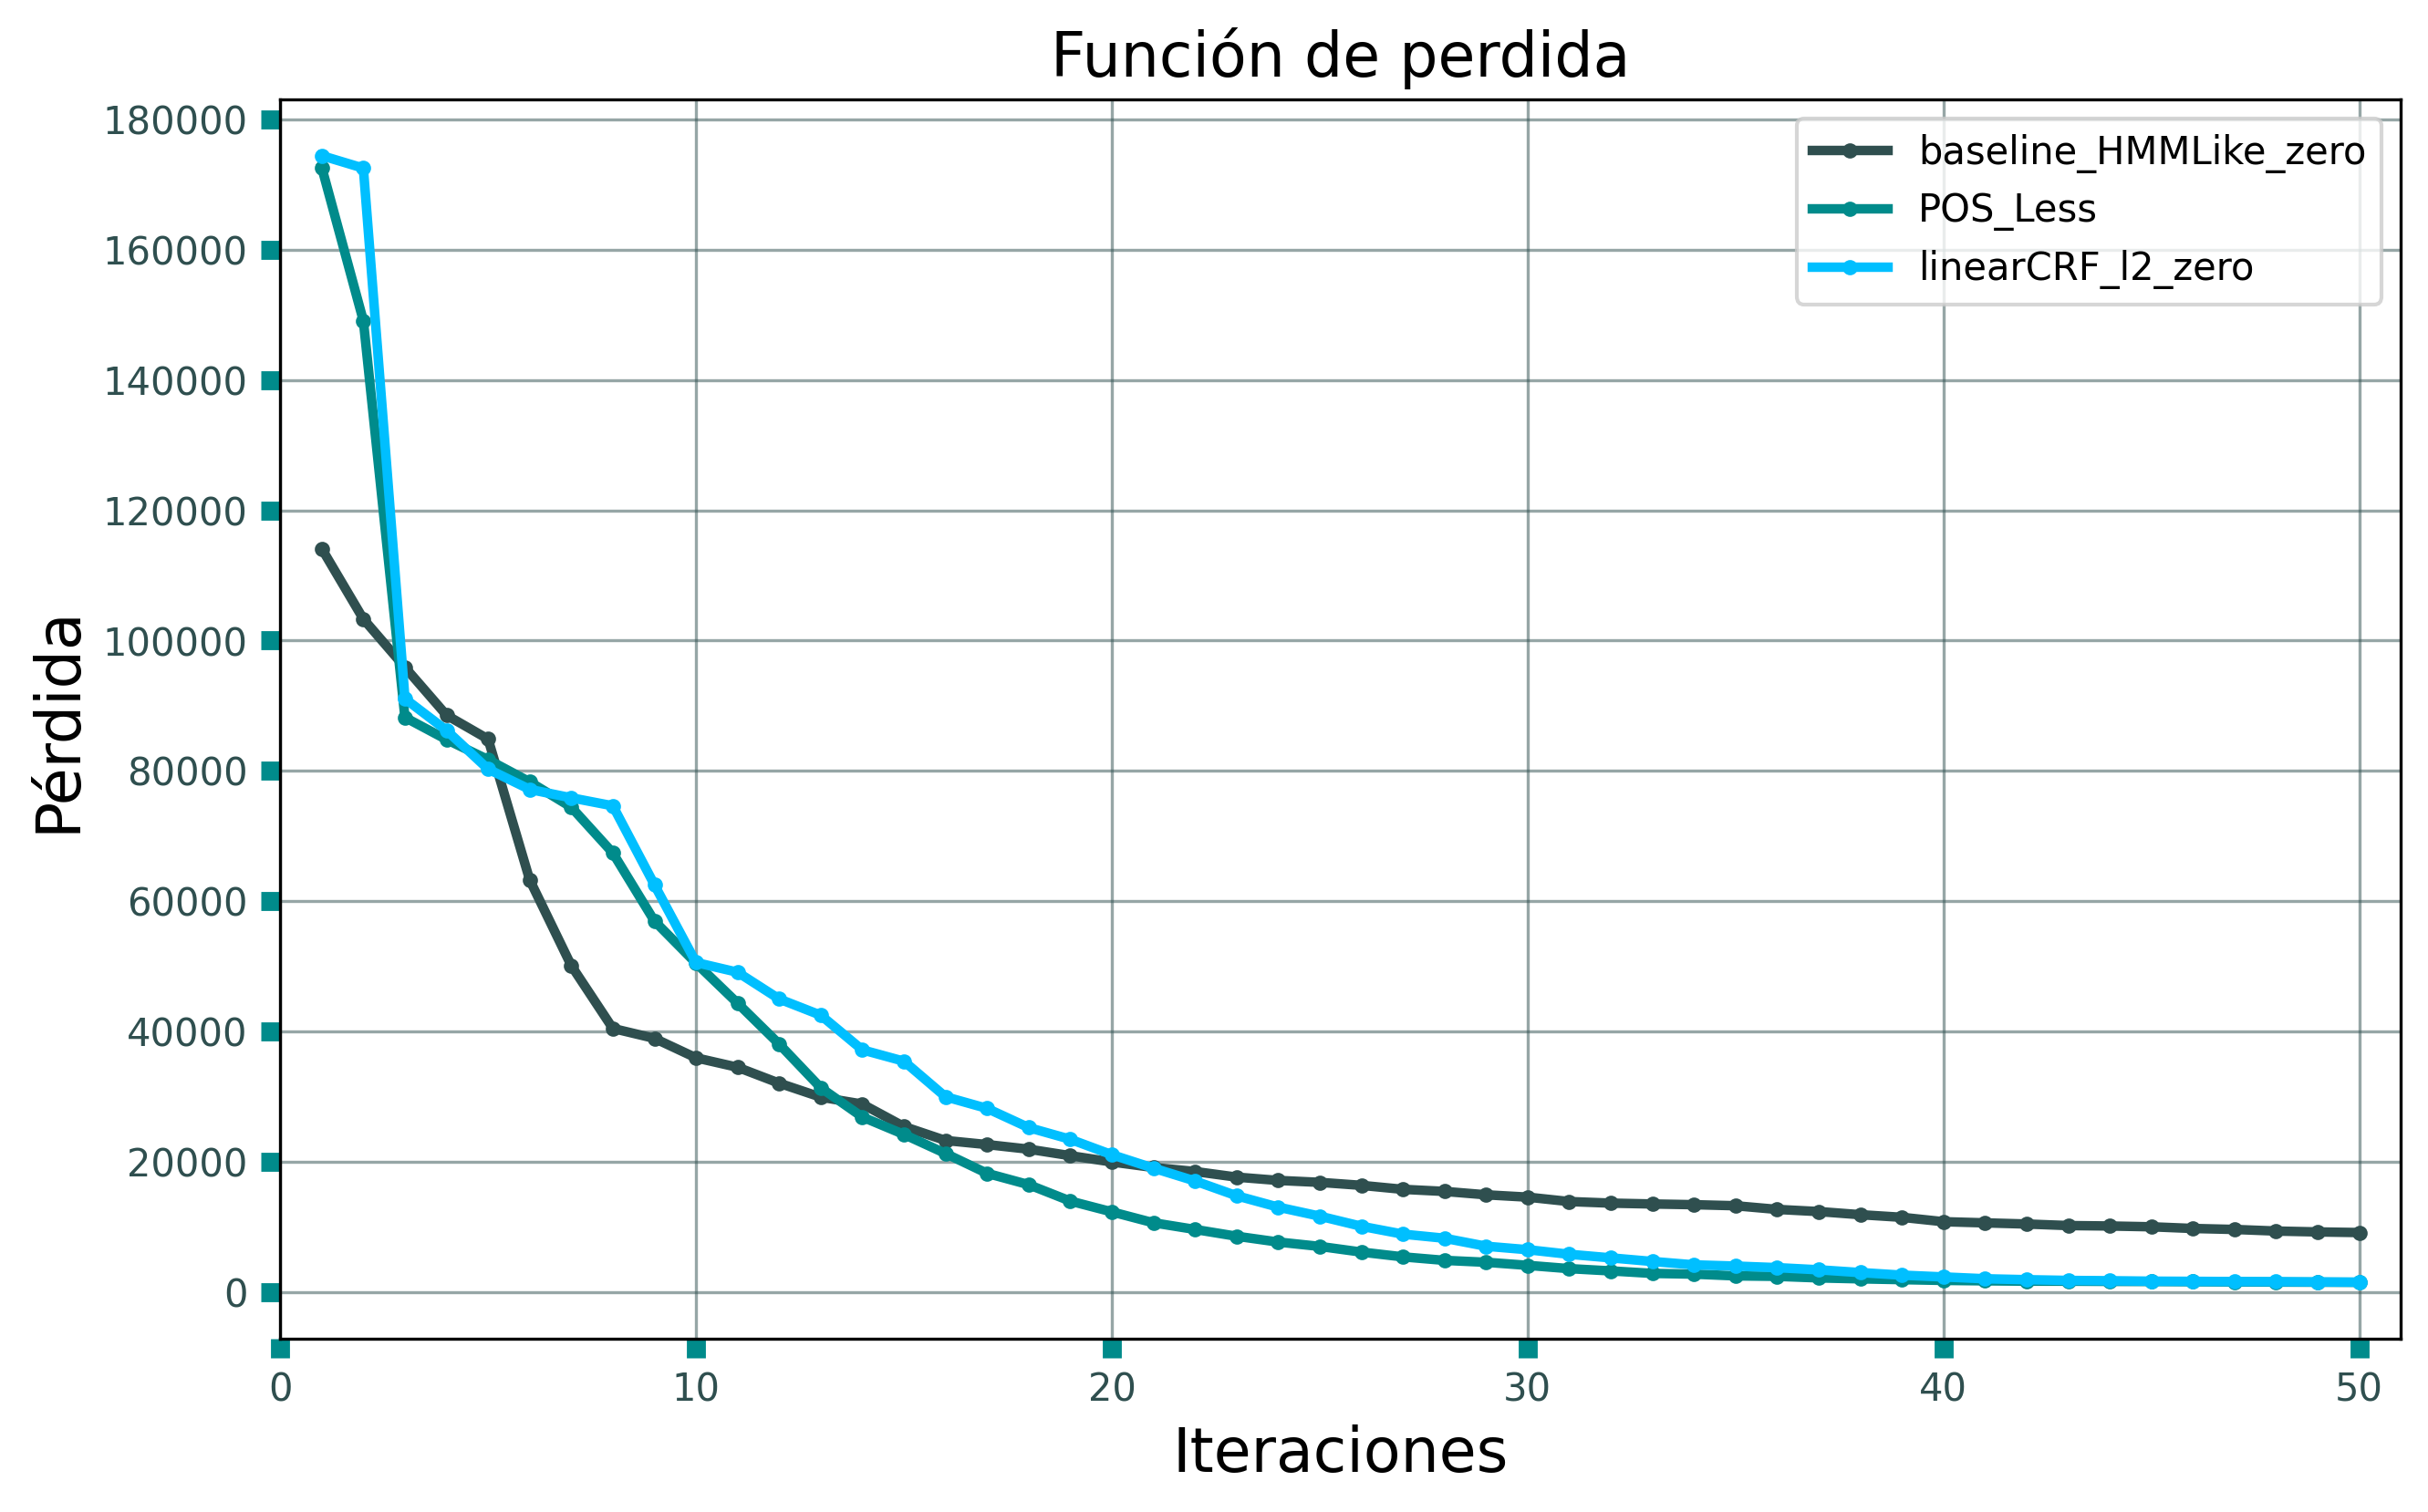
\includegraphics[width=\textwidth]{img/loss_models.png}
	\caption{Función de perdida de los modelos con mejor desempeño}
	\label{fig:loss_models}
\end{figure}

Mostramos una comparación de la función de perdida en la figura \ref{fig:loss_models} de los modelos que se encuentran en la tabla \ref{tab:models-comparation}. En la figura se encuentran las curvas para la iteración $K = 10$ de cada modelo.

En la figura \ref{fig:loss_models} vemos como el modelo \textsf{baseline\_HMMLike\_zero} comienza con una pérdida baja en comparación con los otros dos modelos pero que a medida que avanzan las iteraciones la minimización del error no es tan buena. Esto puede deberse a la cantidad de información codificada en la \textit{feature functions} de inicio.

Por otro lado, las curvas de los modelos \textsf{POS\_Less} y \textsf{linearCRF\_l2\_zero} reflejan un mejor desempeño que la del modelo base. Esto reafirma el desempeño observado en la tabla \ref{tab:models-comparation} que sugiere que a mayor información codificada en las \textit{feature functions} el desempeño es mejor.

La información codificada en ambos modelos es casi la misma salvo por que en los modelos \textsf{POS\_Less} se omitieron las etiquetas \textit{POS}. Ergo, las curvas de los modelos \textsf{POS\_Less} y \textsf{linearCRF\_l2\_zero} son  similares.

En la tabla \ref{tab:tags-linearcrf} se observa la precisión, el \textit{recall} y el \textit{f1-score} que dan información detallada de la eficiencia del modelo \textsf{linearCRF\_l2\_zero} en el etiquetado del último \textit{fold}. Con base en dicha tabla hacemos las siguientes observaciones.

\begin{table}[ht]
    \centering
    \begin{tabular}{| c | c | c | c | c |}\hline
        \textbf{Etiqueta} & \textbf{Precisión} & \textbf{Recall} & \textbf{F1-score} & \textbf{Instancias} \\\hline
        prt & 0.33 & 0.33 & 0.33 & 3\\
        pl & 0.71 & 0.45 & 0.56 & 11\\
        2.cnt & 0.75 & 1 & 0.86 & 3\\
        lig & 0.87 & 0.9 & 0.88 & 29\\
        3.cnt & 0.88 & 0.88 & 0.88 & 8\\
        1.obj & 0.91 & 0.83 & 0.87 & 12\\
        ctrf & 0.95 & 0.95 & 0.95 & 22\\
        stem & 0.96 & 0.96 & 0.96 & 771\\
        prag & 0.97 & 0.97 & 0.97 & 29\\
        3.icp & 0.97 & 0.9 & 0.94 & 40\\\hline
    \end{tabular}
    \caption{Métricas por etiqueta del modelo \textsf{linearCRF\_l2\_zero}}
    \label{tab:tags-linearcrf}
\end{table}

Vemos un bajo desempeño en la etiqueta \textsc{prt} (`partícula') el cual puede deberse a que la etiqueta hace referencia a cosas que no son sistemáticas, que son inusuales o raras y a que \textsc{prt} puede aparecer en cualquier contexto. Además, el bajo \textit{recall} en esta etiqueta puede deberse a que los plurales tienen variaciones en la forma. Por ejemplo algunas palabras plurales tendrán `-hí', o bien `-mí', incluso algunos pocas muestran plural `-phi'.

Por otro lado, las etiquetas como \textsc{stem} (Raíz) o \textsc{ctrf} (`Contrafactual') al ser sistemáticas y muy frecuentes se ven beneficiadas por lo que tienen una \textit{precisión} y un \textit{recall} altos. 

\textsc{prag} (`Pragmático') aparece en los verbos y siempre en la misma posición (al final de la palabra en la posicion del verbo) lo que hace que tambien sea fácilmente predicha por el modelo. Es interesante que este morfema es frecuente pero si se quita no aporta mucha información. Podría decirse que es una muletilla que se traduce como `pues'.

Finalmente, \textsc{3.icp} (`Tercera persona incompletivo'), es un morfema de tiempo muy frecuentemente usado (su equivalencia en español sería el tiempo presente en tercera persona). Siempre aparece antes del verbo y siempre en la misma posición. Por tanto, esta etiqueta es de las mas altas en desempeño.

Cabe destacar que las etiquetas \textsc{stem, prag y 3.icp}, que son las etiquetas con mayor desempeño, no necesariamente comparte la frecuencia. Mientras que \textsc{steam} es la etiqueta con mayor frecuencia \textsc{prag} y \textsc{3.icp} muestran una frecuencia considerablemente mas baja. Aún asi, las tres etiquetas son las que muestran la \textit{precisión}, \textit{recall} y \textit{f1-score} más altos.

En suma, vemos que el modelo tiene dificultades para asignar las etiquetas a frases que no son comunes y que son dependientes \diego{Mas bien que son independientes del contexto ¿no?} del contexto. Contrario, las que tiene alta \textit{precisión} y \textit{recall} son sistemáticas aunque vemos que la frecuencia no es un factor determinante. Entonces, las variaciones morfológicas y las etiquetas con apariciones no sistémicas propician un bajo rendimiento en el etiquetado.

En la tabla \ref{tab:tags-hmmlike} se muestran la \textit{precisión}, el \textit{recall} y el \textit{f1-score} que dan información detallada de la eficiencia del modelo \textsf{baseline\_HMMLike\_zero} en el etiquetado del último \textit{fold}. 

\begin{table}[ht]
    \centering
    \begin{tabular}{| c | c | c | c | c |}\hline
        \textbf{Etiqueta} & \textbf{Precisión} & \textbf{Recall} & \textbf{F1-score} & \textbf{Instancias} \\\hline
        3.imp & 0.33 & 0.33 & 0.33 & 3\\
        med & 0.4 & 1 & 0.57 & 2\\
        mod & 0.43 & 0.21 & 0.29 & 14\\
        dual.exc & 0.5 & 1 & 0.67 & 1\\
        muy & 0.5 & 0.5 & 0.5 & 4\\
        1.prf & 0.57 & 0.8 & 0.67 & 5\\
        2.cnt & 0.6 & 1 & 0.75 & 3\\
        3.prf & 0.6 & 0.75 & 0.67 & 4\\
        loc & 0.62 & 0.83 & 0.71 & 6\\
        3.pls & 0.67 & 1 & 0.8 & 6\\
        stem & 0.83 & 0.81 & 0.82 & 810\\\hline
    \end{tabular}
    \caption{Métricas por etiqueta del modelo \textsf{baseline\_HMMLike\_zero}}
    \label{tab:tags-hmmlike}
\end{table}

Etiquetas como \textsc{dual.exc} (`Dual Exclusivo') y \textsc{med} (`Voz media') tienen un \textit{recall} alto pero una \textit{precisión} baja lo que sugiere que el modelo esta teniendo \textit{overfitting}. En particular, la etiqueta \textsc{med} puede verse afectada también porque aparece con variaciones entre `n-' y `m-'. Notamos que en general el bajo desempeño con estas etiquetas puede deberse a la baja frecuencia de instancias. 

Destacamos que la \textit{precisión} de las etiquetas \textsc{stem} (raíz) es $13\%$ menor que la presente en el modelo \textsf{linearCRF\_l2\_zero} a pesar de tener una frecuencia alta con lo que reafirma que el desempeño de los modelos construidos con \textit{CRFs} se ven beneficiados más por la información de la lengua codificada en las \textit{feature functions} que por la frecuencia de las etiquetas.

Finalmente, el desempeño de etiquetado de este modelo es el más bajo. Dado que tenemos un bajo número de instancias de origen podemos concluir que \textsf{baseline\_HMMLike\_zero} es mas dependiente de la frecuencia que de la estructura. Esto tiene sentido dado que la información estructural dada para la construcción del modelo (a través de las \textit{feature functions}) es mínima.

A continuación mostramos ejemplos de frases etiquetadas en los entornos de experimentación \textsf{linearCRF\_l2\_zero} y \textsf{baseline\_HMMLike\_zero}

\subsubsection{Ejemplos de etiquedado del modelo \textsf{linearCRF\_l2\_zero}}

\begin{exe}
    \ex \gll {b$\mu$} {m-bi-'$\mu$n-gí} {ya} {dó-ráhi-$\iota$-'wi}\\
    {\textsc{stem}} {\textsc{med-3.icp-stem-1.obj}} {\textsc{stem}} {\textsc{1.cpl-stem}}\\
    \trans `Cuando me pegaban pues me quitaba' \label{ejemplo:linearcrf-correcto}
\end{exe}

En el etiquetado \ref{ejemplo:linearcrf-correcto} vemos la aparición de etiquetas sistemáticas como \textsc{stem} y \textsc{3.icp}, por mencionar algunas, por lo que la frase es correctamente etiquetada.

\begin{exe}
\ex \begin{xlist}
    \ex \gll {g-i-né}\\
    {\textbf{\textsc{psd-3.icp}}-\textsc{stem}}\\
    \trans `*Quería' \label{ejemplo:linearcrf-incorrecto-a}
    \ex \gll {gi-né}\\
    {\textsc{2.pot-stem}}\\
    \trans `Vas a querer'\label{ejemplo:linearcrf-correcto-b}
    \end{xlist}
\end{exe}

En el ejemplo \ref{ejemplo:linearcrf-incorrecto-a} se ve como el modelo hace una mala segmentación. Esto puede deberse por un lado a que la etiqueta \textsc{3.icp} es muy frecuente en el corpus y que dado que la etiqueta previa es \textsc{psd} el modelo se inclina por estas etiquetas frecuentes. El patrón \textsc{psd-3.icp} es muy frecuente por lo que el modelo tiende a utilizarlo causando un mal etiquetado. Por otra parte, la combinación correcta de etiquetas (\textsc{2.pot-stem}) es poco frecuente. La versión del etiquetado esperado se puede ver en el ejemplo \ref{ejemplo:linearcrf-correcto-b}

Curiosamente la letra `g' por si misma no coincide con ningún patrón del tiempo pasado pero la letra `i' siguiente si corresponde a un \textsc{3.icp} por lo que el modelo esta haciendo una inferencia regresiva. Como  la letra `i' es \textsc{3.icp} la letra anterior debería ser etiquetada como \textsc{psd}.

Es notorio que en múltiples casos en los que hay morfemas alrededor del verbo el modelo tiende a considerarlos parte del \textsc{stem} en lugar de separarlos. Esto quiere decir que toma morfemas que no deberían ser parte del \textsc{stem}. Tiene sentido en tanto que el \textsc{stem} no tiene una forma determinada (es una clase abierta) y puede tener cualquier combinación de letras. Un ejemplo de esto se puede ver en la glosa \ref{ejemplo:stem-erroneo}.

Las características de las clases abiertas las hacen difíciles de ver por completo en el entrenamiento contrario a las clases cerradas que con clases finitas. Además, notamos que el modelo \textsf{linearCRF\_zero\_l2} se equivoca cuando no hay suficiente contexto, por ejemplo, frases cortas de una sola palabra.

\begin{exe}
\ex \begin{xlist}
    \ex \gll {bi-nd$\mu$zú}\\
    {\textbf{\textsc{3.cpl-stem}}}\\
    \trans (No traducible con esta segmentación)\label{ejemplo:stem-erroneo}
    \ex \gll {bi-nd$\mu$-zú}\\
            {3.icp-muy-stem} \\
        \trans 'Se asustó'
    \end{xlist}
\end{exe}


\subsubsection{Ejemplo de frase etiquetada por el modelo \textsf{baseline\_HMMLike\_zero}}

\Diego{Revisar el error y la frase}
\begin{exe} 
    \ex \gll {bi-'{\mu}n-gi} {y{\iota}} {mb{\mu}hi} {nge} {hín} {dí-má-né} {gwa-porá} {nge} {dí-má-dáhní}\\
    {\textsc{3.cpl-stem-1.obj}} {\textsc{det.pl}} {\textsc{stem}} {\textsc{stem}} {\textsc{stem}} {\textsc{1.icp-ctrf-stem}} {\textsc{1.icp.irr-stem}} {\textsc{stem}} {\textsc{1.icp-ctrf-stem}}\\
    \trans `Me pegaron los patrones porque no me quería apurar, porque era flojo'
    \label{ejemplo:hmmlike-correcto}
\end{exe} 

Ya mencionamos que el desempeño de este modelo, que simula un \textit{HMM}, depende de la frecuencia. El ejemplo \ref{ejemplo:hmmlike-correcto} muestra etiquetas y patrones muy frecuentes como \textsc{cpl} y \textsc{ctrf} que en general son también sistemáticos. A pesar de que el etiquetador pertenece al entorno con menor información y desempeño el etiquetado es correcto. Además, ayuda que, como se observo, los ejemplos largos son mejores para estos modelos de baja información.

\begin{exe}
    \ex \begin{xlist}
        \ex \gll {má-ndé} {bi-ni}\\
        {\textbf{\textsc{ctrf-stem}}} {\textsc{3.cpl-stem}}\\
        \trans `*La tarde lo tuve' \label{ejemplo:hmmlike-incorrecto-a}
        \ex \gll {mánde} {bi-ni}\\
        {\textsc{stem}} {\textsc{3.cpl-stem}}\\
        \trans `Ayer lo tuve' \label{ejemplo:hmmlike-incorrecto-b}
        \end{xlist}
\end{exe}

En el ejemplo \ref{ejemplo:hmmlike-incorrecto-a} vemos como el modelo está sobre ajustado ya que el morfema `ma' está siendo asociado con la etiqueta \textsc{ctrf} dado que esta combinación es muy frecuente. Incluso el morfema `ndé' es un \textsc{stem} existente y válido pero incorrecto en este contexto. Notamos que ocurre el efecto contrario a lo que vimos en el ejemplo \ref{ejemplo:stem-erroneo}. Esto es que ya que ha visto el morfema `ma' separado con tanta frecuencia en este ejemplo también lo separa en lugar de integrarlo en uno solo y etiquetarlo como \textsc{stem}.

Un error característico de este modelo es que esta sobre segmentando y encontrando morfemas que no son correctos. Confunde secuencias con patrones frecuentes y no es raro por que a este modelo se le otorgó mínima información por lo que no esta tomando tanto en cuenta el contexto de las oraciones. Con mas información esto se reduce.

Por último, notamos que en este entorno de experimentación los modelos no aprenden a formar correctamente las estructuras válidas de las \textit{BIO Labels} para generar la glosa. Esto es que la primera etiqueta debe comenzar con una letra \code{`B'} (\textit{Beginning}) seguida opcionalmente de etiquetas que comienzan con la letra \code{`I'} (\textit{Inside}). Mostramos una la salida de etiquetas generadas por el modelo en el ejemplo \ref{ejemplo:estructura-glosa-errona}.

\begin{exe}
    \ex \gll {i} {b} {i} {t} {h} {ó} {p} {a} {n} {$\iota$} {r} {$\iota$} {c} {h} {á} {i}\\
    {\textbf{\textsc{I-it}}} {\textsc{B-3.cpl}} {\textsc{I-3.cpl}} {\textbf{\textsc{B-ila}}} {\textbf{\textsc{I-ila}}} {\textbf{\textsc{I-ila}}} {\textsc{B-stem}} {\textsc{I-stem}} {\textbf{\textsc{B-stem}}} {\textbf{\textsc{I-stem}}} {\textsc{B-det}} {\textsc{I-det}} {\textsc{B-stem}} {\textsc{I-stem}} {\textsc{I-stem}}  {\textsc{I-stem}}\\\label{ejemplo:estructura-glosa-errona}
\end{exe}

Como podemos ver la primera etiqueta comienza con una letra \code{`I'} cuando debería ser una \code{`B'}. En concreto la salida con las \textit{BIO  Labels} bien formadas sería la que se ve en el ejemplo \ref{ejemplo:estructura-glosa-correcta}.

\begin{exe}
    \ex \gll {i} {b} {i} {t} {h} {ó} {p} {a} {n} {$\iota$} {r} {$\iota$} {c} {h} {á} {i}\\
    {\textsc{B-stem}} {\textsc{B-3.cpl}} {\textsc{I-3.cpl}} {\textsc{B-stem}} {\textsc{I-stem}} {\textsc{I-stem}} {\textsc{B-stem}} {\textsc{I-stem}} {\textsc{B-det}} {\textsc{I-det}} {\textsc{B-det}} {\textsc{I-det}} {\textsc{I-det}} {\textsc{B-stem}} {\textsc{I-stem}} {\textsc{I-stem}}\\\label{ejemplo:estructura-glosa-correcta}
\end{exe}

Con las \textit{BIO Labels} que se muestran en el ejemplo \ref{ejemplo:estructura-glosa-correcta} se tendría la glosa que se muestra en el ejemplo \ref{ejemplo:frase-glosada}.

\begin{exe}
    \ex \gll {i} {bi-thó} {pa} {n$\iota$} {r$\iota$} {chái}\\
    {\textsc{stem}} {\textsc{3.cpl-stem}} {\textsc{stem}} {\textsc{det}} {\textsc{det}} {\textsc{stem}}\\
    \trans `Y paso por una zanaja'\label{ejemplo:frase-glosada}
\end{exe}

\Diego{Hacer una recapitulacion del ejemplo donde se equivoca para dar cierre}


\chapter{Conclusiones}

La información lingüística codificada en las fuature functions es muy importante para mejorar el desempeño del etiquetador

Sin embargo, las etiquetas pos no son restrictivas 
\Ximena{el hecho de no necesitar las pos es bueno para las lenguas minorizadas pues no siempre hay etiquetadores automáticos para estas lenguas}

Cuando se le quita información al modelo en las \textit{feature functions} la frecuencia de las instancias tiene mayor pero. Por lo tanto, para bajos recursos, donde las frecuencias de las instancias son bajas, es necesario dar un contexto más amplio y agregar información lingüística mas detallada.

\section{Trabajo Futuro}

Poner en un ambiente de transferencia y probar si los modelos que entrene pueden aplicarse a otras variantes de otomí con un zero show learning

\bibliography{barriga_tesis}
	
\end{document}
